%
% This is an example LaTeX file which uses the SANDreport class file.
% It shows how a SAND report should be formatted, what sections and
% elements it should contain, and how to use the SANDreport class.
% It uses the LaTeX article class, but not the strict option.
% ItINLreport uses .eps logos and files to show how pdflatex can be used
%
% Get the latest version of the class file and more at
%    http://www.cs.sandia.gov/~rolf/SANDreport
%
% This file and the SANDreport.cls file are based on information
% contained in "Guide to Preparing {SAND} Reports", Sand98-0730, edited
% by Tamara K. Locke, and the newer "Guide to Preparing SAND Reports and
% Other Communication Products", SAND2002-2068P.
% Please send corrections and suggestions for improvements to
% Rolf Riesen, Org. 9223, MS 1110, rolf@cs.sandia.gov
%
\documentclass[pdf,12pt]{INLreport}
% pslatex is really old (1994).  It attempts to merge the times and mathptm packages.
% My opinion is that it produces a really bad looking math font.  So why are we using it?
% If you just want to change the text font, you should just \usepackage{times}.
% \usepackage{pslatex}
\usepackage{times}
\usepackage[FIGBOTCAP,normal,bf,tight]{subfigure}
\usepackage{amsmath}
\usepackage{amssymb}
\usepackage{soul}
\usepackage{pifont}
\usepackage{enumerate}
\usepackage{listings}
\usepackage{fullpage}
\usepackage{xcolor}          % Using xcolor for more robust color specification
\usepackage{ifthen}          % For simple checking in newcommand blocks
\usepackage{textcomp}
\usepackage{mathtools}
\usepackage{relsize}
\usepackage{lscape}
\usepackage[toc,page]{appendix}
\usepackage{RAVEN}

\newtheorem{mydef}{Definition}
\newcommand{\norm}[1]{\lVert#1\rVert}
%\usepackage[table,xcdraw]{xcolor}
%\usepackage{authblk}         % For making the author list look prettier
%\renewcommand\Authsep{,~\,}

% Custom colors
\definecolor{deepblue}{rgb}{0,0,0.5}
\definecolor{deepred}{rgb}{0.6,0,0}
\definecolor{deepgreen}{rgb}{0,0.5,0}
\definecolor{forestgreen}{RGB}{34,139,34}
\definecolor{orangered}{RGB}{239,134,64}
\definecolor{darkblue}{rgb}{0.0,0.0,0.6}
\definecolor{gray}{rgb}{0.4,0.4,0.4}

\lstset {
  basicstyle=\ttfamily,
  frame=single
}


\setcounter{secnumdepth}{5}
\lstdefinestyle{XML} {
    language=XML,
    extendedchars=true,
    breaklines=true,
    breakatwhitespace=true,
%    emph={name,dim,interactive,overwrite},
    emphstyle=\color{red},
    basicstyle=\ttfamily,
%    columns=fullflexible,
    commentstyle=\color{gray}\upshape,
    morestring=[b]",
    morecomment=[s]{<?}{?>},
    morecomment=[s][\color{forestgreen}]{<!--}{-->},
    keywordstyle=\color{cyan},
    stringstyle=\ttfamily\color{black},
    tagstyle=\color{darkblue}\bf\ttfamily,
    morekeywords={name,type},
%    morekeywords={name,attribute,source,variables,version,type,release,x,z,y,xlabel,ylabel,how,text,param1,param2,color,label},
}
\lstset{language=python,upquote=true}

\usepackage{titlesec}
\newcommand{\sectionbreak}{\clearpage}
\setcounter{secnumdepth}{4}

%\titleformat{\paragraph}
%{\normalfont\normalsize\bfseries}{\theparagraph}{1em}{}
%\titlespacing*{\paragraph}
%{0pt}{3.25ex plus 1ex minus .2ex}{1.5ex plus .2ex}

%%%%%%%% Begin comands definition to input python code into document
\usepackage[utf8]{inputenc}

% Default fixed font does not support bold face
\DeclareFixedFont{\ttb}{T1}{txtt}{bx}{n}{9} % for bold
\DeclareFixedFont{\ttm}{T1}{txtt}{m}{n}{9}  % for normal

\usepackage{listings}

% Python style for highlighting
\newcommand\pythonstyle{\lstset{
language=Python,
basicstyle=\ttm,
otherkeywords={self, none, return},             % Add keywords here
keywordstyle=\ttb\color{deepblue},
emph={MyClass,__init__},          % Custom highlighting
emphstyle=\ttb\color{deepred},    % Custom highlighting style
stringstyle=\color{deepgreen},
frame=tb,                         % Any extra options here
showstringspaces=false            %
}}


% Python environment
\lstnewenvironment{python}[1][]
{
\pythonstyle
\lstset{#1}
}
{}

% Python for external files
\newcommand\pythonexternal[2][]{{
\pythonstyle
\lstinputlisting[#1]{#2}}}

\lstnewenvironment{xml}
{}
{}

% Python for inline
\newcommand\pythoninline[1]{{\pythonstyle\lstinline!#1!}}

% Named Colors for the comments below (Attempted to match git symbol colors)
\definecolor{RScolor}{HTML}{8EB361}  % Sonat (adjusted for clarity)
\definecolor{DPMcolor}{HTML}{E28B8D} % Dan
\definecolor{JCcolor}{HTML}{82A8D9}  % Josh (adjusted for clarity)
\definecolor{AAcolor}{HTML}{8D7F44}  % Andrea
\definecolor{CRcolor}{HTML}{AC39CE}  % Cristian
\definecolor{RKcolor}{HTML}{3ECC8D}  % Bob (adjusted for clarity)
\definecolor{DMcolor}{HTML}{276605}  % Diego (adjusted for clarity)
\definecolor{PTcolor}{HTML}{990000}  % Paul

\def\DRAFT{} % Uncomment this if you want to see the notes people have been adding
% Comment command for developers (Should only be used under active development)
\ifdefined\DRAFT
  \newcommand{\nameLabeler}[3]{\textcolor{#2}{[[#1: #3]]}}
\else
  \newcommand{\nameLabeler}[3]{}
\fi
\newcommand{\alfoa}[1] {\nameLabeler{Andrea}{AAcolor}{#1}}
\newcommand{\cristr}[1] {\nameLabeler{Cristian}{CRcolor}{#1}}
\newcommand{\mandd}[1] {\nameLabeler{Diego}{DMcolor}{#1}}
\newcommand{\maljdan}[1] {\nameLabeler{Dan}{DPMcolor}{#1}}
\newcommand{\cogljj}[1] {\nameLabeler{Josh}{JCcolor}{#1}}
\newcommand{\bobk}[1] {\nameLabeler{Bob}{RKcolor}{#1}}
\newcommand{\senrs}[1] {\nameLabeler{Sonat}{RScolor}{#1}}
\newcommand{\talbpaul}[1] {\nameLabeler{Paul}{PTcolor}{#1}}
% Commands for making the LaTeX a bit more uniform and cleaner
\newcommand{\TODO}[1]    {\textcolor{red}{\textit{(#1)}}}
\newcommand{\xmlAttrRequired}[1] {\textcolor{red}{\textbf{\texttt{#1}}}}
\newcommand{\xmlAttr}[1] {\textcolor{cyan}{\textbf{\texttt{#1}}}}
\newcommand{\xmlNodeRequired}[1] {\textcolor{deepblue}{\textbf{\texttt{<#1>}}}}
\newcommand{\xmlNode}[1] {\textcolor{darkblue}{\textbf{\texttt{<#1>}}}}
\newcommand{\xmlString}[1] {\textcolor{black}{\textbf{\texttt{'#1'}}}}
\newcommand{\xmlDesc}[1] {\textbf{\textit{#1}}} % Maybe a misnomer, but I am
                                                % using this to detail the data
                                                % type and necessity of an XML
                                                % node or attribute,
                                                % xmlDesc = XML description
\newcommand{\default}[1]{~\\*\textit{Default: #1}}
\newcommand{\nb} {\textcolor{deepgreen}{\textbf{~Note:}}~}


%%%%%%%% End comands definition to input python code into document

%\usepackage[dvips,light,first,bottomafter]{draftcopy}
%\draftcopyName{Sample, contains no OUO}{70}
%\draftcopyName{Draft}{300}

% The bm package provides \bm for bold math fonts.  Apparently
% \boldsymbol, which I used to always use, is now considered
% obsolete.  Also, \boldsymbol doesn't even seem to work with
% the fonts used in this particular document...
\usepackage{bm}


% Define tensors to be in bold math font.
\newcommand{\tensor}[1]{{\bm{#1}}}

% Override the formatting used by \vec.  Instead of a little arrow
% over the letter, this creates a bold character.
\renewcommand{\vec}{\bm}

% Define unit vector notation.  If you don't override the
% behavior of \vec, you probably want to use the second one.
\newcommand{\unit}[1]{\hat{\bm{#1}}}
% \newcommand{\unit}[1]{\hat{#1}}

% Use this to refer to a single component of a unit vector.
\newcommand{\scalarunit}[1]{\hat{#1}}

% \toprule, \midrule, \bottomrule for tables
\usepackage{booktabs}

% \llbracket, \rrbracket
\usepackage{stmaryrd}

\usepackage{hyperref}
\hypersetup{
    colorlinks,
    citecolor=black,
    filecolor=black,
    linkcolor=black,
    urlcolor=black
}

% Compress lists of citations like [33,34,35,36,37] to [33-37]
\usepackage{cite}

% If you want to relax some of the SAND98-0730 requirements, use the "relax"
% option. It adds spaces and boldface in the table of contents, and does not
% force the page layout sizes.
% e.g. \documentclass[relax,12pt]{SANDreport}
%
% You can also use the "strict" option, which applies even more of the
% SAND98-0730 guidelines. It gets rid of section numbers which are often
% useful; e.g. \documentclass[strict]{SANDreport}

% The INLreport class uses \flushbottom formatting by default (since
% it's intended to be two-sided document).  \flushbottom causes
% additional space to be inserted both before and after paragraphs so
% that no matter how much text is actually available, it fills up the
% page from top to bottom.  My feeling is that \raggedbottom looks much
% better, primarily because most people will view the report
% electronically and not in a two-sided printed format where some argue
% \raggedbottom looks worse.  If we really want to have the original
% behavior, we can comment out this line...
\raggedbottom
\setcounter{secnumdepth}{5} % show 5 levels of subsection
\setcounter{tocdepth}{5} % include 5 levels of subsection in table of contents

% ---------------------------------------------------------------------------- %
%
% Set the title, author, and date
%
\title{RAVEN User Guide}
%\author{%
%\begin{tabular}{c} Author 1 \\ University1 \\ Mail1 \\ \\
%Author 3 \\ University3 \\ Mail3 \end{tabular} \and
%\begin{tabular}{c} Author 2 \\ University2 \\ Mail2 \\ \\
%Author 4 \\ University4 \\ Mail4\\
%\end{tabular} }


\author{
\\Andrea Alfonsi
\\Cristian Rabiti
\\Diego Mandelli
\\Joshua Cogliati
\\Congjian Wang
\\Paul W. Talbot
\\Daniel P. Maljovec
\\Curtis Smith
}
%Just people who actually ``developed'' a significant capability in the code should be placed here. Andrea
%\author{\textbf{\textit{Main Developers:}}  \\Andrea Alfonsi}
%\affil{Idaho National Laboratory, Idaho Falls, ID 83402}
%\\\{cristian.rabiti, andrea.alfonsi, joshua.cogliati, diego.mandelli, robert.kinoshita, ramazan.sen\}@inl.gov}

% There is a "Printed" date on the title page of a SAND report, so
% the generic \date should [WorkingDir:]generally be empty.
\date{}


% ---------------------------------------------------------------------------- %
% Set some things we need for SAND reports. These are mandatory
%
\SANDnum{INL/EXT-16-38178}
\SANDprintDate{March 2017}
\SANDauthor{Andrea Alfonsi, Cristian Rabiti, Diego Mandelli, Joshua Cogliati, Congjian Wang, Paul W. Talbot, Daniel P. Maljovec, Curtis Smith}
\SANDreleaseType{Revision 2 draft}


% ---------------------------------------------------------------------------- %
% Include the markings required for your SAND report. The default is "Unlimited
% Release". You may have to edit the file included here, or create your own
% (see the examples provided).
%
% \include{MarkOUO} % Not needed for unlimted release reports

\def\component#1{\texttt{#1}}

% ---------------------------------------------------------------------------- %
\newcommand{\systemtau}{\tensor{\tau}_{\!\text{SUPG}}}

% Added by Sonat
\usepackage{placeins}
\usepackage{array}

\newcolumntype{L}[1]{>{\raggedright\let\newline\\\arraybackslash\hspace{0pt}}m{#1}}
\newcolumntype{C}[1]{>{\centering\let\newline\\\arraybackslash\hspace{0pt}}m{#1}}
\newcolumntype{R}[1]{>{\raggedleft\let\newline\\\arraybackslash\hspace{0pt}}m{#1}}

% end added by Sonat
% ---------------------------------------------------------------------------- %
%
% Start the document
%

\begin{document}

    \maketitle

    % ------------------------------------------------------------------------ %
    % An Abstract is required for SAND reports
    %
%    \begin{abstract}
%    \input abstract
%    \end{abstract}


    % ------------------------------------------------------------------------ %
    % An Acknowledgement section is optional but important, if someone made
    % contributions or helped beyond the normal part of a work assignment.
    % Use \section* since we don't want it in the table of context
    %
%    \clearpage
%    \section*{Acknowledgment}



%	The format of this report is based on information found
%	in~\cite{Sand98-0730}.


    % ------------------------------------------------------------------------ %
    % The table of contents and list of figures and tables
    % Comment out \listoffigures and \listoftables if there are no
    % figures or tables. Make sure this starts on an odd numbered page
    %
    \cleardoublepage		% TOC needs to start on an odd page
    \tableofcontents
    %\listoffigures
    %\listoftables


    % ---------------------------------------------------------------------- %
    % An optional preface or Foreword
%    \clearpage
%    \section*{Preface}
%    \addcontentsline{toc}{section}{Preface}
%	Although muggles usually have only limited experience with
%	magic, and many even dispute its existence, it is worthwhile
%	to be open minded and explore the possibilities.


    % ---------------------------------------------------------------------- %
    % An optional executive summary
    %\clearpage
    %\section*{Summary}
    %\addcontentsline{toc}{section}{Summary}
    %\input{Summary.tex}
%	Once a certain level of mistrust and skepticism has
%	been overcome, magic finds many uses in todays science



%	and engineering. In this report we explain some of the
%	fundamental spells and instruments of magic and wizardry. We
%	then conclude with a few examples on how they can be used
%	in daily activities at national Laboratories.


    % ---------------------------------------------------------------------- %
    % An optional glossary. We don't want it to be numbered
%    \clearpage
%    \section*{Nomenclature}
%    \addcontentsline{toc}{section}{Nomenclature}
%    \begin{description}
%          \item[alohomoral]
%           spell to open locked doors and containers
%          \item[leviosa]
%           spell to levitate objects
%    \item[remembrall]
%           device to alert you that you have forgotten something
%    \item[wand]
%           device to execute spells
%    \end{description}


    % ---------------------------------------------------------------------- %
    % This is where the body of the report begins; usually with an Introduction
    %
    \SANDmain		% Start the main part of the report

\section{Introduction}
% High-level RAVEN description
RAVEN~\cite{alfonsiMC} ~\cite{alfonsiPSA}~\cite{RAVENFY13}~\cite{ESREL2014} is a software framework that allows the user to perform parametric and stochastic
analysis based on the response of complex system codes.
The initial development was designed to provide dynamic probabilistic risk analysis
capabilities (DPRA) to the thermal-hydraulic code RELAP-7~\cite{relap7FY12}, currently under development
at Idaho National Laboratory (INL).
Now, RAVEN is not only a framework to perform DPRA but it is a
multi-purpose stochastic and uncertainty quantification platform, capable of communicating with any system code.

This report serves as a theoretical manual for selected algorithms implemented within the RAVEN framework. 
It is intended to provide some theorectical treatments of the selected algorithms in the areas of sensitivity
and uncertainty analysis, reduced order modeling, statistical analysus, data mining and DPRA that can help the
user to understand the theory behind the key concepts.


\section{Introduction}

\section{Introduction}
\subsection{System Purpose}

RAVEN is a flexible and multi-purpose uncertainty quantification (UQ), regression analysis, probabilistic risk assessment 
(PRA), data analysis and model optimization software.  Depending on the tasks to be accomplished and on the 
probabilistic
 characterization of the problem, RAVEN perturbs (Monte-Carlo, latin hyper-cube, reliability surface search, etc.) the
 response of the system under consideration by altering its own parameters. The system is modeled by third party
 software (RELAP5-3D, MAAP5, BISON, etc.) and accessible to RAVEN either directly (software coupling) or
 indirectly (via input/output files). The data generated by the sampling process is analyzed using classical statistical
 and more advanced data mining approaches. RAVEN also manages the parallel dispatching (i.e. both on
 desktop/workstation and large High-Performance Computing machines) of the software representing the physical 
 model. RAVEN heavily relies on artificial intelligence algorithms to construct surrogate models of complex physical
 systems in order to perform uncertainty quantification, reliability analysis (limit state surface) and parametric studies.

\subsection{System Scope}

RAVEN’s scope is to provide a set of capabilities to build analysis flows based on UQ, PRA, Optimization and Data Analysis techniques to be applied to any physical model(s). The main objective of the software is to assist the engineer/user to:
\begin{itemize}
  \item identify the best design (on any physics/model), its safety and confidence;
  \item estimate the likelihood of undesired outcomes (risk analysis);
  \item identify main drivers/events to act on for reducing impact/consequences of anomalous dynamic behaviors of the 
         system under analysis;
  \item to construct analysis flows combining multiple physical models and analysis procedures.
\end{itemize}

In other words, the RAVEN software is aimed to be employed for:
\begin{itemize}
  \item Uncertainty Quantification;
  \item Sensitivity Analysis / Regression Analysis;
  \item Probabilistic Risk and Reliability Analysis (PRA);
  \item Data Mining Analysis;
  \item Model Optimization.
\end{itemize}

The combination of all the previously mentioned analysis capabilities is a key component to 
define safety margins in engineering design that are more representative of real prediction deficiencies. 
This could reduce 
cost and maintain a more coherent safety level of the system (no excess/no lack of safety margins in any operational 
condition).
The risk analysis, assisted by the data mining algorithms, is used to find engineering solutions to reduce costs, while 
preserving safety margins, or to increase safety at the minimum cost. These tasks can be automatically achieved by using 
optimization algorithms available in the RAVEN software.
Moreover, the knowledge of the relationship between input and system response uncertainties allows identifying effective 
experiments, which are the most suitable for increasing the accuracy of the model. This approach reduces time and cost 
of the deployment of complex engineering systems and new technologies.

The RAVEN software employs several novel and unique techniques, based on extensive usage of artificial intelligence 
algorithms, such as adaptive (smart) sampling, adaptive branching algorithms (Dynamic Event Tree), time-dependent 
statistical analysis and data mining. 
The overall set of algorithms implemented in the RAVEN software are designed to handle highly non-linear systems, 
characterized by system response discontinuities and discrete variables. These capabilities are crucial for handling 
complex system models, such as nuclear power plants.
For example, reliability surface analysis, as implemented in RAVEN, is unique and capable to handle non-linear, 
discontinuous systems, allowing for faster and more accurate assessing of failure risk for complex systems.

In addition, the RAVEN software provides the unique capability to combine any model (e.g. physical models, surrogate 
models, data analysis models, etc.) in a single entity (named Ensemble Model) where each model can feedback into others. This capability allows the user to analyze system that could be simulated only by using complex computational work-flows.

\subsection{User Characteristics}

The users of the RAVEN software are expected to be part of any of the
following categories:
\begin{itemize}
  \item \textbf{Core developers (RAVEN core team)}: These are the developers of the RAVEN software. They will be responsible for following
    and enforcing the appropriate software development standards. They will be responsible for designing, implementing and 
    maintaining the software.
  \item \textbf{External developers}: A Scientist or Engineer that utilizes the RAVEN framework and wants to extend its capabilities (new interface to external
 applications, new data analysis tecniques, new sampling strategies, etc).This user will typically have a background in modeling and 
simulation techniques and/or numerical analysis but may only have a limited skill-set when it comes to object-oriented coding, C++/Python languages.
  \item \textbf{Analysts}:  These are users that will run the code and perform various analysis on the simulations they perform. These users may interact with developers of the system requesting new features and reporting bugs found and will typically make heavy use of the input file format.
\end{itemize}


\subsection{Software infrastructure}
\subsubsection{Outlines}
RAVEN has been developed in a highly modular and pluggable way in order to enable easy integration of different programming languages (i.e., C++, Python) and, as already mentioned, coupling with any system code.

\subsubsection{Probabilistic and Parametric framework}
The probabilistic and parametric framework represents the core of the RAVEN analysis capabilities. The main idea behind the design of the system is the creation of a multipurpose framework characterized by high flexibility with respect to the possible performable analysis. The framework must be capable of constructing the analysis/calculation flow at run-time, interpreting the user-defined instructions and assembling the different analysis tasks following a user specified scheme.
In order to achieve such flexibility, combined with reasonably fast development, a programming language naturally suitable for this kind of approach was needed: $Python$.


\begin{figure}[ht]
  \centering
  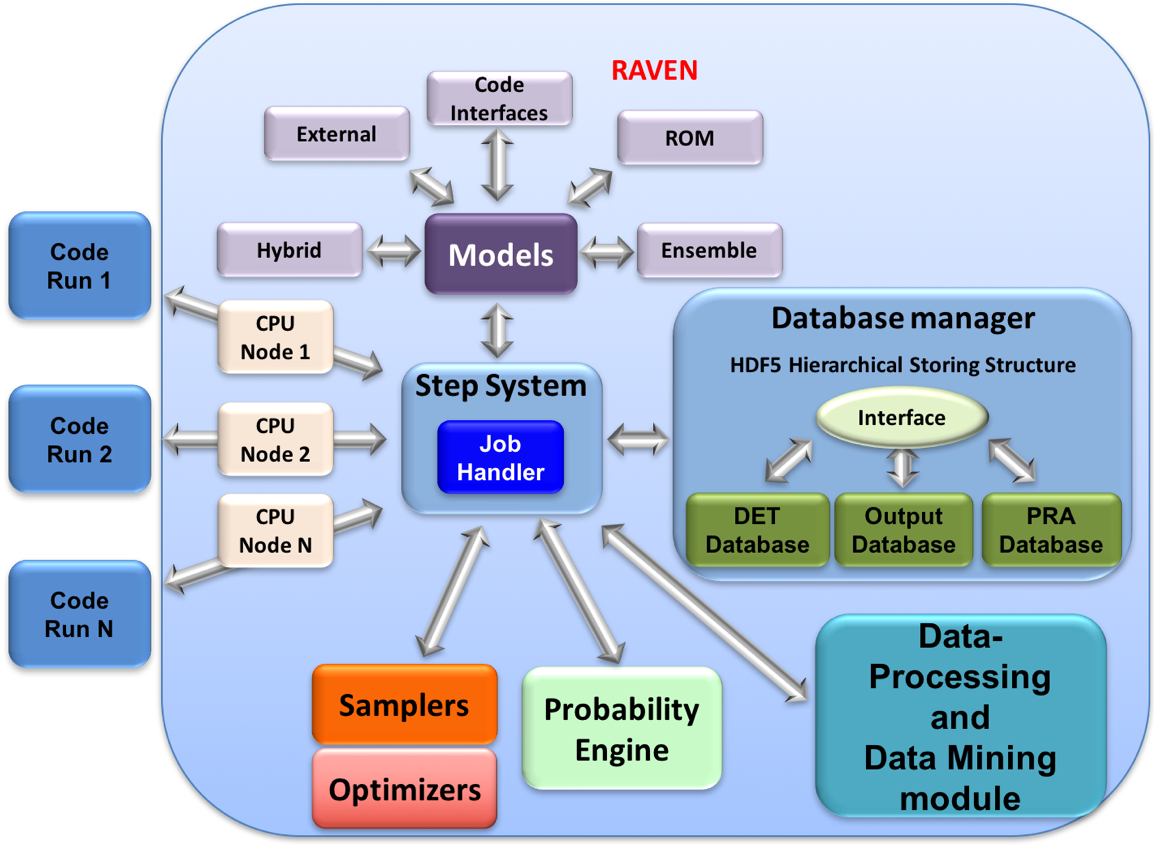
\includegraphics[width=1.0\textwidth]  {pics/RavenFramework.png}
  \caption{RAVEN framework layout}
  \label{fig:RAVENframeworkLayout}
\end{figure}

Hence, RAVEN is coded in $Python$ and is characterized by an object-oriented design. The core of the analysis performable through RAVEN is represented by a set of basic components (objects) the user can combine, in order to create a custom analysis flow. A list of these components and a summary of their most important functionalities are reported as follows:
\begin{itemize}
\item	Distribution: In order to explore the input/output space, RAVEN requires the capability to perturb the input space (initial conditions and/or model coefficients of a system code). The input space is generally characterized by probability distribution functions (PDFs), which might need to be considered when a perturbation is applied. In this respect, a large library of PDFs is available.
\item Sampler: A proper approach to sample the input space is fundamental for the optimization of the computational time. In RAVEN, a ``sampler'' employs a unique perturbation strategy that is applied to the input space of a system. The input space is defined through the connection of uncertain variables and their relative probability distributions.
\item Model: A model is the representation of a physical system (e.g. Nuclear Power Plant); it is therefore capable of predicting the evolution of a system given a coordinate set in the input space. In addition it can represent an
action on a data in order to extract key features (e.g. Data mining).
\item Reduced Order Model (ROM): The evaluation of the system response, as a function of the coordinates in the input space, is very computationally expensive, especially when brute-force approaches (e.g. Monte Carlo methods) are chosen as the sampling strategy. ROMs are used to lower this cost, reducing the number of needed points and prioritizing the area of the input space that needs to be explored. They can be considered as an artificial representation of the link between the input and output spaces for a particular system.
\end{itemize}
The list above is not comprehensive of all the RAVEN framework components (visualization and storage infrastructure).
\\ Figure~\ref{fig:RAVENframeworkLayout} shows a schematic representation of the whole framework, highlighting the communication pipes among the different modules and engines. As can be seen, in the figure all the components reported above are schematically shown. In addition the data management, mining and processing modules are shown.

\subsubsection{Distribution}
As already mentioned, the perturbation of the input space, through the initial conditions (parameters) affected by uncertainties, needs to be performed by the proper distribution functions. RAVEN provides, through an interface to the BOOST library, the following variate (truncated and not) distributions: Bernoulli, Binomial, Exponential, Logistic, Lognormal, Normal, Poisson, Triangular, Uniform, Weibull, Gamma, and Beta.
\\The usage of uni-variate distributions for sampling initial conditions is based on the assumption that the uncertain parameters are not correlated with each other. Quite often uncertain parameters are subject to correlations and thus the uni-variate approach is not applicable. This happens when a generic outcome is dependent on different phenomena simultaneously (i.e. the outcome dependency description can not be collapsed to a function of a single variable). RAVEN currently supports both N-dimensional (N-D) PDFs. The user can provide the distribution values on either Cartesian or sparse grid, which determines the interpolation algorithm used in the evaluation of the imported CDF/PDF:
\begin{enumerate}
\item N-Dimensional Spline, for Cartesian grids
\item Inverse weight, for sparse grids
\end{enumerate}
Internally, RAVEN provides the needed N-D differentiation and integration algorithms to compute the PDF from the CDF and vice-versa.
\\As already mentioned, the sampling methods use the distributions in order to perform probability-weighted perturbations. For example, in the Monte Carlo approach, a random number $\in [0,1]$ is generated (probability threshold) and the CDF, corresponding to that probability, is inverted in order to retrieve the parameter value usable in the simulation. The existence of the inverse for variate distributions is guaranteed by the monotonicity of the CDF. For N-D distributions this condition is not sufficient since the $CDF(X)\longrightarrow [0,1],X \in  R^{N} $ and therefore it could not be a bijective function. From an application point of view, this means the inverse of a N-D CDF is not unique.
\\As an example, the Figure~\ref{fig:NDDistributionExample} shows a multivariate normal distribution for a pipe failure as function of the pressure and temperature. The plane identifies an isoprobability surface (in this case, a line) that represents a probability threshold of 50 \% in this example.  Hence, the inverse of this CDF is an infinite number of points.
 \\As easily inferable, the standard sampling approach cannot directly be employed. When multivariate distributions are used, RAVEN implements a surface search algorithm for identifying the iso-probability surface location. Once the location of the surface has been found, RAVEN chooses, randomly, one point on it.

\begin{figure}
  \centering
  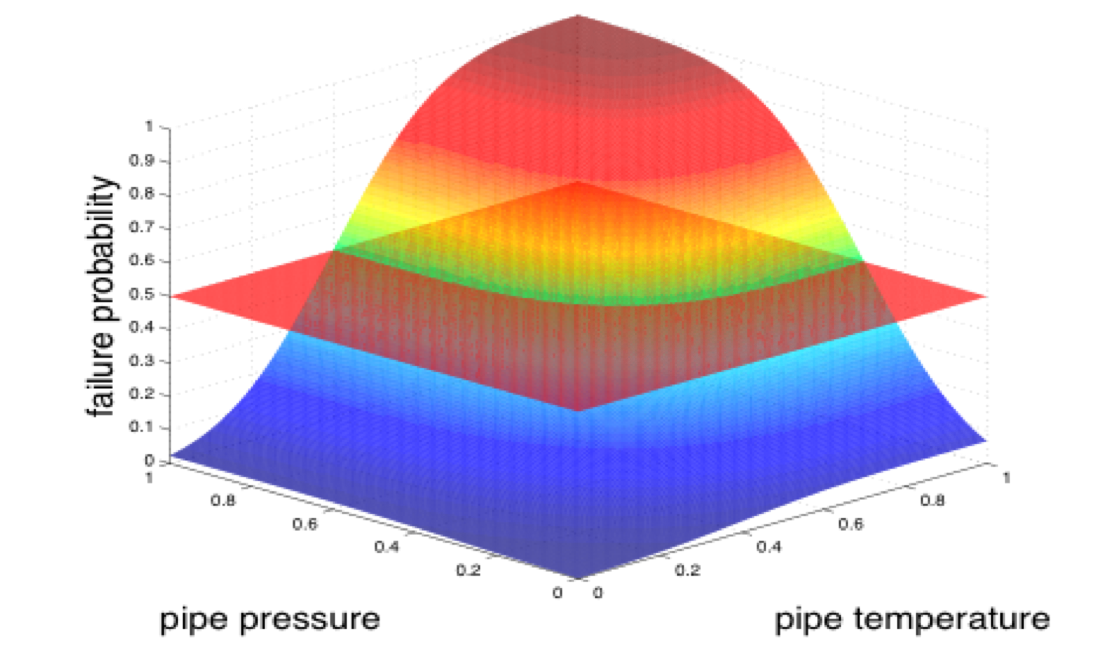
\includegraphics[width=0.5\textwidth]  {pics/NDimensionalDistributionExample.png}
  \caption{2-D CDF, function of pressure and temperature}
  \label{fig:NDDistributionExample}
\end{figure}

\subsubsection{Sampler}

The sampler is probably the most important entity in the RAVEN framework. Indeed, it performs the driving of the specific sampling strategy and, hence, determines the effectiveness of the analysis, from both an accuracy and computational point of view.  The samplers, that are available in RAVEN, can be categorized in three main classes:
\begin{itemize}
 \item Forward
 \item Dynamic Event Tree (DET)
 \item Adaptive
\end{itemize}
\paragraph{Forward Samplers} ~\\
The Forward sampler category collects all the strategies that perform the sampling of the input space without exploiting, through dynamic learning approaches, the information made available from the outcomes of calculation previously performed (adaptive sampling) and the common system evolution (patterns) that different sampled calculations can generate in the phase space (dynamic event tree).
In the RAVEN framework, several different and well-known forward samplers are available:
\begin{itemize}
\item Monte Carlo (MC)
\item Stratified based, whose most known specialization is the Latin Hyper-Cube Sampling (LHS)
\item Grid Based
\item Response Surface Design of Experiment
\item Sparse Grid
\item Factorials
\item Etc.
\end{itemize}
As already mentioned, all these sampling strategies are well known, as well as their properties. Therefore, a detailed investigation of their application is not provided.
%%%%%%%%%%%%%%%%%%%%%%%%%%%%%%%%%%%%%%%%%%%%%%%%%%%%%%%%%%%%%%%%%%%%%%%%%%%%%%%%
\paragraph{Dynamic Event Tree Samplers}~\\
In order to clarify the idea behind the Dynamic Event Tree Sampler currently available in RAVEN, a small overview is needed.
\\In technological complex systems, as nuclear power plants, an accident scenario begins with an initiating event and then evolves over time through the interaction of dynamics and stochastic events. This mutual action leads to the production of infinitely many different scenarios, which define a continuous dynamic event tree with infinite branches. At each time point, the stochastic variability of the accident outcomes is determined by a multivariate probability distribution. The PRA analysis needs an approximation to this distribution for selected consequence variables. A way to achieve this goal is an Event Tree approach. In dynamic PRA analysis, Conventional Event Tree sequences are run simultaneously starting from a single initiating event. The branches occur at user specified times and/or when an action is required by the operator and/or the system, creating a deterministic sequence of events based on the time of their occurrence. One of the disadvantages of this method is that the timing/sequencing of events and system dynamics is not explicitly accounted for in the analysis. In order to overcome these limitations a “dynamic” approach is needed. The Dynamic Event Tree (DET) technique brings several advantages, among which is the fact that it simulates probabilistic system evolution in a way that is consistent with the severe accident model. This leads to a more realistic and mechanistically consistent analysis of the system taken into consideration. The dynamic PRA, in general, and the Dynamic Event Tree methodologies in particular, are designed to take the timing of events explicitly into account, which can become very important especially when uncertainties in complex phenomena are considered. Hence, the main idea of this methodology is to let a system code determine the pathway of an accident scenario.
\\From an application point of view, a N-D grid is built on the CDF space. A single simulation is spawned and a set of triggers is added to the system code control logic. Every time a trigger gets activated (one of the CDF thresholds in the grid is violated), a new set of simulations (branches) is spawned. Each branch carries its own probability.
\\Figure \ref{fig:DETschemeExample} shows a practical example. In this particular case, it is assumed that the
probability failure of a pipe depends on the fluid pressure magnitude. Three probability thresholds are defined on
the cumulative distribution function. One simulation is spawned (0). As soon as the pressure of the fluid reaches a
value corresponding to a 33\% probability (CDF), a stop signal is sent and the framework starts two new
simulations (branches). The branch in which the system evolved to the newer condition (pipe failed, red line)
carries 33\% of the probability, while the other the complementary amount. The same procedure is repeated at
point 2.
\\Generally, not all the input space can be explored using a DET approach. For instance, usually the parameters affected by aleatory uncertainty are sampled using a dynamic event tree approach, while the ones characterized by epistemic uncertainty are sampled through ``forward'' sampling strategies.
\\As already mentioned, this strategy requires a tight interaction between the system code and the sampling driver (i.e., RAVEN framework). In addition, the system code must have a control logic capability (i.e. trigger system). For these reasons, the application of this sampling approach to a generic code needs a larger effort when compared to the other Samplers available in RAVEN. Currently, the DET is fully available for the thermal-hydraulic codes RELAP-7 and RELAP5-3D.
\\In the RAVEN framework, several different DET-based samplers are available:
\begin{itemize}
\item Dynamic Event Tree (aleatory sampling);
\item Hybrid Dynamic Event Tree (aleatory and epistemic sampling);
\item Adaptive Dynamic Event Tree (goal-oriented sampling for aleatory sampling);
\item Adaptive Hybrid Dynamic Event Tree (goal-oriented sampling for aleatory and epistemic sampling).
\end{itemize}

\begin{figure}
  \centering
  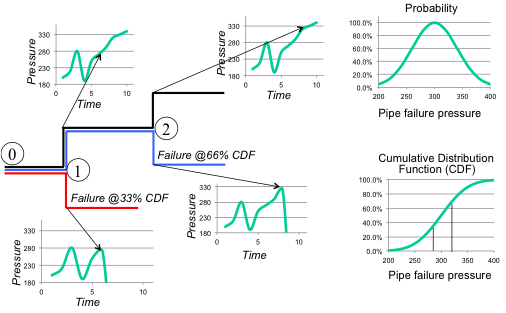
\includegraphics[width=0.7\textwidth]  {pics/DETscheme.png}
  \caption{Dynamic Event Tree simulation pattern}
  \label{fig:DETschemeExample}
\end{figure}

%%%%%%%%%%%%%%%%%%%%%%%%%%%%%%%%%%%%%%%%%%%%%%%%%%%%%%%%%%%%%%%%%%%%%%%%%%%%%%%%
\paragraph{Adaptive Samplers}~\\
A key feature available within RAVEN is the possibility to perform smart sampling (also known as adaptive sampling) as an alternative to classical ``forward'' techniques.
\\The motivation is that nuclear simulations are often computationally expensive, time-consuming, and high dimensional with respect to the number of input parameters. Thus, exploring the space of all possible simulation outcomes is unfeasible using finite computing resources. During simulation-based probabilistic risk analysis, it is important to discover the relationship between a potentially large number of input parameters and the output of a simulation using as few simulation trials as possible.
\\This is a typical context for performing adaptive sampling where a few observations are obtained from the simulation, a reduced order model (ROM) is built to represent the simulation space, and new samples are selected based on the model constructed. The ROM is then updated based on the simulation results of the sampled points. In this way, it is attempted to gain the most information possible with a small number of carefully selected sampled points, limiting the number of expensive trials needed to understand features of the system space.
\\In the RAVEN framework, several different adaptive samplers are available:
\begin{itemize}
\item Limit Surface Search;
\item Adaptive Dynamic Event Tree;
\item Adaptive Hybrid Dynamic Event Tree ;
\item Adaptive Sparse Grid;
\item Adaptive Sobol Decomposition.
\end{itemize}

\subsubsection{Models}
The Model entity, in the RAVEN environment, represents a ``connection pipeline'' between the input and the output space. The RAVEN framework does not own any physical model (i.e. it does not posses the equations needed to simulate a generic physical system, such as Navier-Stocks equations, Maxwell equations, etc.), but implements Application Program Interfaces (APIs) by which any generic model can be integrated and interrogated. The RAVEN framework provides APIs for four different model categories: Codes, Externals, Post-Processors (PPs) and Reduced Order Models (ROMs). In the following paragraphs, a brief explanation of each of this Model categories is reported.
\paragraph{Code} ~\\
The \textit{Code} model represents the communication pipe between the RAVEN framework and any system and physical code. The communication between RAVEN and any driven code is performed through the implementation of interfaces directly operated by the framework.
\\The procedure of coupling a new code/application with RAVEN is a straightforward process. The coupling is performed through a \textit{Python}  interface that interprets the information coming from RAVEN and translates them to the input of the driven code. The coupling procedure does not require modifying RAVEN itself. Instead, the developer creates a new \textit{Python} interface that is going to be embedded in RAVEN at run-time (no need to introduce hard-coded coupling statements).  This interface needs to be placed in a folder (whatever name) located in (see figure~\ref{fig:CodeInterfaceLocation}):
\begin{lstlisting}[language=bash]
 path/to/raven/distribution/raven/framework/CodeInterfaces/
\end{lstlisting}

\begin{figure}
  \centering
  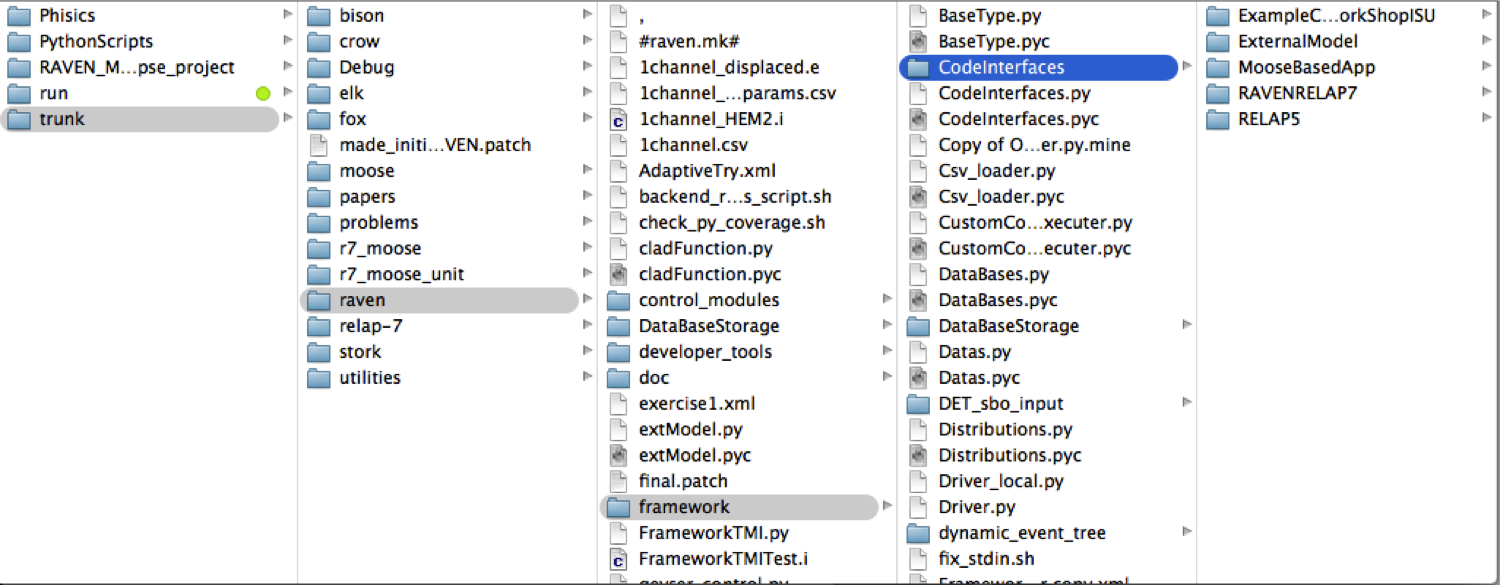
\includegraphics[width=0.8\textwidth]  {pics/CodeInterfaceLocation.png}
  \caption{Code Interface Location}
  \label{fig:CodeInterfaceLocation}
\end{figure}
At the initialization stage, RAVEN imports all the Interfaces that are contained in this directory and performs some preliminary cross-checks.
\\ If the coupled code is parallelized and/or multi-threaded, RAVEN is going to manage the system in order to optimize the computational resources in both workstations and High Performance Computing systems.
\\Currently, RAVEN has APIs for RELAP5-3D, RELAP-7, any MOOSE-based application, SASS and Modelica.
\paragraph{External Model} ~\\
The External model allows the user to create, in a \textit{Python} file (imported, at run-time, in the RAVEN framework), its own model (e.g. set of equations representing a physical model, connection to another code, control logic, etc.). This model will be interpreted/used by the framework and, at run-time, will become part of RAVEN itself.
\paragraph{Post-Processor} ~\\
The Post-Processor model represents the container of all the post-processing capabilities in the RAVEN code. This model is aimed to process the data (for example, derived from the sampling of a physical code) in order to identify representative Figure of Merits. This system has  been designed and, presently, is under heavy development by the whole RAVEN team.  Currently, the following post-processors are available:
\begin{itemize}
 \item \textit{Basic Statistics}, container of the algorithms to compute many of the most important statistical quantities. This post-processor is able to compute mean, sigma/variance, variation coefficient, skewness, kurtosis, median, percentiles and all the principal matrix quantities such as covariance, sensitivity (either leas-squared and variance weighted) and correlation matrices;
 \item \textit{Comparison Statistics}, aimed to employ validation and verification metrics;
 \item \textit{Limit Surface}, aimed to compute the limit surface in the input space (i.e. the hyper-surface that represents the boundary between the failure/success of the system);
 \item \textit{Limit Surface Integral}, intended to compute the integral of the limit surface that corresponds to the probability of failure;
  \item \textit{Safest Point}, provides the coordinates of the farthest point from the limit surface that is given as an input. The safest point coordinates are expected values of the coordinates of the farthest points from the limit surface in the space of the ``controllable'' variables based on the probability distributions of the ``non-controllable'' variables. The term ``controllable'' identifies those variables that are under control during the system operation, while the ``non-controllable'' variables are stochastic parameters affecting the system behavior randomly;
 \item \textit{External Post-Processor}, user-defined post-processor;
 \item \textit{Topological Decomposition}, aimed to compute an approximated hierarchical Morse-Smale complex which will add two columns to a data-set, performing a topological decomposition of such data-set;
 \item \textit{Data Mining}, container of all the RAVEN data mining, clustering and dimensionality reduction techniques aimed to identify dominant and common patterns in high-dimensionality data.
\end{itemize}
\paragraph{Reduced Order Model} ~\\
 As briefly mentioned, a ROM is a mathematical representation of a system, used to predict a selected output space of a physical system.
The ``training'' is a process that uses sampling of the physical model to improve the prediction capability (capability to predict the status of the system given a realization of the input space) of the ROM. More specifically, in RAVEN the Reduced Order Model is trained to emulate a high fidelity numerical representation (system codes) of the physical system. Two general characteristics of these models can be generally assumed (even if exceptions are possible):
\begin{enumerate}
   \item The higher the number of realizations in the training sets, the higher is the accuracy of the prediction performed by the reduced order model. This statement is true for most of the cases although some ROMs might be subject to the over-fitting issues. The over-fitting phenomenon is not discussed here, since its occurrence is highly dependent on the algorithm type, (and there is large number of ROM options available in RAVEN). Every time the user chooses a particular reduced order model algorithm to use, he should consult the relative literature;
   \item The smaller the size of the input domain with respect to the variability of the system response, the more likely the surrogate model will be able to represent the system output space.
\end{enumerate}
In most of the cases of interest, the information that is sought is related to defining the failure boundaries of a system with respect to perturbations in the input space. For this reason, in the development of RAVEN, it has been given priority to the introduction of a class of supervised learning algorithms, which are usually referred to as classifiers. A classifier is a reduced order model that is capable of representing the system behavior through a binary response (failure/success).
\\The first class of classifier introduced has been the Support Vector Machines (SVMs) [reference] with several different kernels (polynomial of arbitrary integer order, radial basis function kernel, sigmoid) followed by a nearest-neighbor based classification using a K-D tree search algorithm. Currently, RAVEN supports around 40 different ROM methodologies. All these supervised learning algorithms have been imported via an API from the scikit-learn [reference] library. In addition, the N-Dimensional spline and the inverse weight methods, that are currently available for the interpolation of N-Dimensional PDF/CDF, can also be used as ROMs.
\subsubsection{Simulation Environment}
RAVEN is perceived by the user as a pool of tools and data. Any action in which the tools are applied to the data is considered a calculation ``step'' in the RAVEN environment. Simplistically, a ``step'' can be seen as a \textbf{transfer function} between the input and output space through a Model (e.g. Code, External, ROM or Post-Processor). One of the most important step in the RAVEN framework is called ``multi-run'', that is aimed to handle calculations that involve multiple runs of a driven code (sampling strategies). Firstly, the RAVEN input file associates the variables to a set of PDFs and to a sampling strategy. The ``multi-run'' step is used to perform several runs in a block of a model (e.g. in a MC sampling).
\begin{figure}[ht]
  \centering
  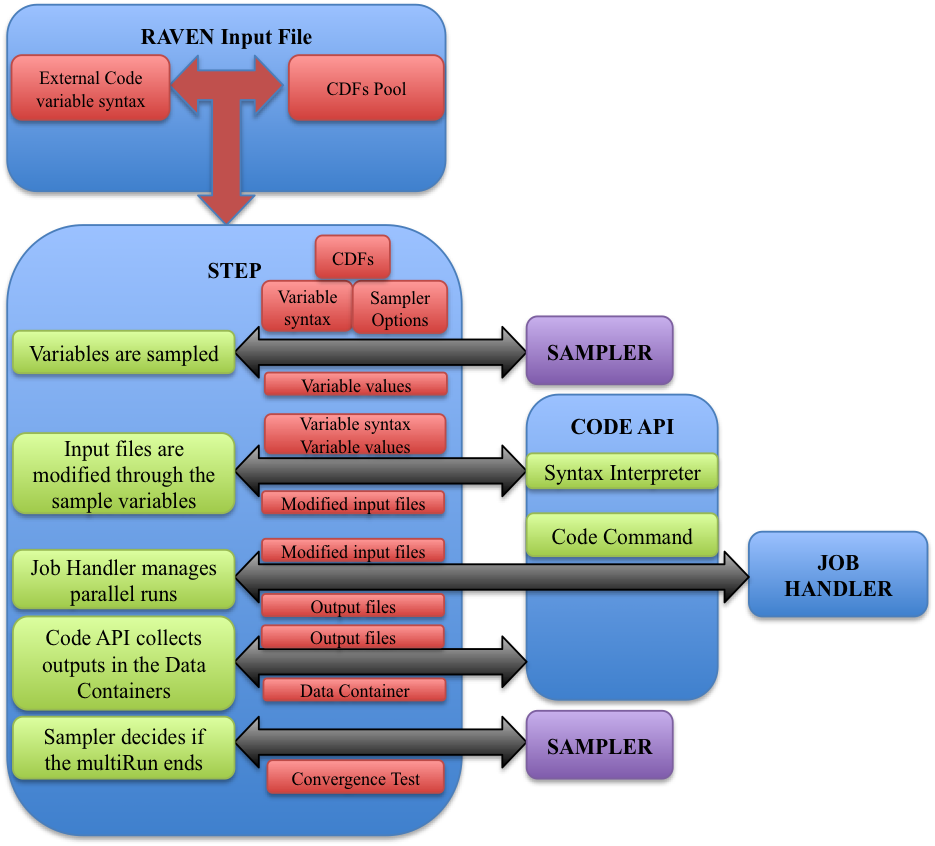
\includegraphics[width=0.8\textwidth]  {pics/MultiRunCalculationFlow.png}
  \caption{Calculation flow for a multi-run sampling}
  \label{fig:multiRun}
\end{figure}
At the beginning of each sub sequential run, the sampler provides the new values of the variables to be perturbed. The code API places those values in the input file. At this point, the code API generates the run command and asks to be queued by the job handler. The job handler manages the parallel execution of as many runs as possible within a user prescribed range and communicates with the step controller when a new set of output files are ready to be processed. The code API receives the new input files and collects the data in the RAVEN internal format. The sampler is queried to assess if the sequence of runs is ended, if not, the step controller asks for a new set of values from the sampler and the sequence is restarted as described in Figure~\ref{fig:multiRun}.
The job handler is currently capable to run different run instances of the code in parallel and can also handle codes that are multi-threaded or using any form of parallel implementation.
RAVEN also has the capability to plot the simulation outcomes while the set of sampling is performed and to store the data for later recovery.

\section{Raven Input Structure}
The RAVEN code does not have a fixed calculation flow, since all of its basic
objects can be combined in order to create a user-defined calculation flow.
%
Thus, its input (XML format) is organized in different XML blocks, each with a
different functionality.
%
The main input blocks are as follows:
\begin{itemize}
  \item \xmlNode{Simulation}: The root node containing the
  entire input, all of
  the following blocks fit inside the \emph{Simulation} block.
  %
  \item \xmlNode{RunInfo}: Specifies the calculation
  settings (number of parallel simulations, etc.).
  %
  \item \xmlNode{Files}: Specifies the files to be
  used in the calculation.
  %
  \item \xmlNode{Distributions}: Defines distributions
  needed for describing parameters, etc.
  %
  \item \xmlNode{Samplers}: Sets up the strategies used for
  exploring an uncertain domain.
  %
  \item \xmlNode{Optimizers}: Sets up the strategies used for
  minimizing/maximizing an objective function.
  %
  \item \xmlNode{DataObjects}: Specifies internal data objects
  used by RAVEN.
  %
  \item \xmlNode{Databases}: Lists the HDF5 databases used
  as input/output to a
  RAVEN run.
  %
  \item \xmlNode{OutStreams}: Visualization and
  Printing system block.
  %
  \item \xmlNode{Models}: Specifies codes, ROMs,
  post-processing analysis, etc.
  %
  \item \xmlNode{Functions}: Details interfaces to external
  user-defined functions and modules.
  %
  the user will be building and/or running.
  %
  \item \xmlNode{Steps}: Combines other blocks to detail a
  step in the RAVEN workflow including I/O and computations to be performed.
  %
\end{itemize}

Each of these blocks are explained in dedicated sections in the following
chapters.
%
\subsection{Comments}
Comments may be included in the RAVEN input using standard XML comments,
using \verb|<!--| and \verb|-->| as shown in the example below.
\begin{lstlisting}[style=XML]
<Simulation>
  ...
  <!-- An Example Comment -->
  <Samplers>
  ...
\end{lstlisting}
Comments may be placed anywhere \emph{except} before the \xmlNode{Simulation}
node or after the \xmlNode{/Simulation} node.
%
Comments outside the root node will cause errors in maintaining input file
compatability.
%
Additionally, comments must completely surround any nodes they comment out.
%
Comments are intended to completely remove blocks of code, or to add readability.
%
For instance, the following is INCORRECT usage:
\begin{lstlisting}[style=XML]
  <!--<Assembler> -->
  <!--</Assembler> -->
\end{lstlisting}
%
and the following is compatible usage for a code block:
%
\begin{lstlisting}[style=XML]
  <!--<Samplers>
    <Monte Carlo name='mc'>
      ...
    </Monte Carlo>
    ...
  </Samplers> -->
\end{lstlisting}


\subsection{Verbosity}
\label{sec:verbosity}
Each block within RAVEN also makes use of a \xmlAttr{verbosity} system,
which allows a user to control the level of output to the user interface.
These settings are declared globally as attributes in the \xmlNode{Simulation} node,
and locally in each block.  The verbosity levels are
\begin{itemize}
\item \xmlString{silent} - Only simulation-breaking errors are displayed.
\item \xmlString{quiet} - Errors as well as warnings are displayed.
\item \xmlString{all} (default) - Errors, warnings, and messages are displayed.
\item \xmlString{debug} - For developers. All errors, warnings, messages, and debug messages are displayed.
\end{itemize}
Examples of verbosity usage are included in many examples throughout this manual.

At the \xmlNode{Simulation} node, the following global variables can be set:
\begin{itemize}
  \item \xmlAttr{verbosity}, optional string, determines the global verbosity level.  Defaults to
    \xmlString{all}.
  \item \xmlAttr{printTimeStamps}, optional boolean, determines whether time stamps will be added to printed
    messages.  Defaults to true.
  \item \xmlAttr{color}, optional boolean, determines whether ANSI color tags will be used in printed
    messages.  Defaults to false.
  \item \xmlAttr{profile}, optional comma-separated list, enables time profiling of parts of RAVEN.  Options
    include \xmlString{jobs}.  Default is no profiling.
\end{itemize}


\subsection{External Input Files}
The \xmlNode{ExternalXML} node defines external input file (XML format) that can be used to replace any XML nodes
under \xmlNode{Simulation} in the RAVEN input file. This node allows a user to load any external input file that contains
the required XML nodes into the RAVEN input file. Each \xmlNode{ExternalXML} node has the following attributes:
\begin{itemize}
\item \xmlAttr{node}, \xmlDesc{required string attribute}, user-defined XML node of RAVEN input file.
\item \xmlAttr{xmlToLoad}, \xmlDesc{required string attribute}, file name with its absolute or relative path. Note: if a
relative path is specified, it must be relative with respect to the RAVEN input file.
\end{itemize}
%
For example, if the file \texttt{Models.xml} contain the required RAVEN input XML node \xmlNode{Models},
the RAVEN input file might appear as:
%
\begin{lstlisting}[style=XML,morekeywords={node,xmlToLoad}]
<Simulation>
  ...
  <Steps>
    ...
  </Steps>
  ...
  <ExternalXML node='Models' xmlToLoad='external_input/Models.xml'/>
  ...
</Simulation>
\end{lstlisting}
%
Another example, if the file \texttt{MultiRun.xml} contain the required RAVEN input XML node \xmlNode{MultiRun}
under node \xmlNode{Steps}, the RAVEN input file might appear as:
\begin{lstlisting}[style=XML,morekeywords={node,xmlToLoad}]
<Simulation>
  ...
  <Steps>
    ...
    <ExternalXML node='MultiRun' xmlToLoad='external_input/MultiRun.xml'/>
    ...
  </Steps>
  ...
</Simulation>
\end{lstlisting}

\input{manualFormats.tex}
\input{manualStructure.tex}
\subsection{Build RAVEN input: \xmlNode{SingleRun}}
\label{sub:singleRun}
In this section, we will show the user how to use RAVEN to run a single instance of a driven code, and
printing some variables. 
We will start to build a very simple RAVEN input, and this input file can be found at 
``\textit{raven/tests/framework/user\textunderscore guide/ravenTutorial/singleRun.xml}''. 
From this process, we hope the user can get a better idea about
RAVEN entities and learn how to build their own RAVEN inputs for their applications.
In order to accomplish these tasks, the following procedures are needed:
\begin{enumerate}
   \item \textbf{Set up the running environment}: \xmlNode{RunInfo}
     \\The \textbf{RunInfo} entity is an information container which describes how the overall computation should
      be performed. This Entity accepts several input settings that define how to drive the calculation and set up,
      when needed, particular settings for the machine the code needs to run on (queue system, if not Portable
      Batch System-PBS, etc.). For the simple case, the \textbf{RunInfo} will look like:
      \xmlExample{framework/user_guide/ravenTutorial/singleRun.xml}{RunInfo}
      In this specific case, only one step named \xmlString{single} is going to be sequentially run using a single
      processor as defined by \xmlNode{BatchSize}. All the output files and temporary files will be dumped in the
      folder \xmlString{singleRunAnalysis}.

   \item \textbf{Provide the required files}: \xmlNode{Files}
     \\ The \textbf{Files} entity  defines any files that might be needed within the RAVEN run. This could include
     inputs to the Model, pickled ROM files, or Comma Separated Value (CSV) files for post-processors, to name a few.
     Each entry in the \xmlNode{Files} block is a tag with the file type. Files given through the input XML at this
     point are all \xmlNode{Input} type. Each \xmlNode{Input} node has a required attributes \xmlAttr{name}. It does
     not need to be the actual filename, and it is the name by which RAVEN will use to identify the specific file. Other
     optional attributes are not directly used by RAVEN, and they are mainly used by the \textbf{CodeInterface}. More
     detailed information can be found in the user manual ~\cite{RAVENuserManual}. For the simple case, the \textbf{Files}
     will look like:
     \xmlExample{framework/user_guide/ravenTutorial/singleRun.xml}{Files}
     This RAVEN input file shows that the user will provide a file that is located at ``\textit{../commonFiles/referenceInput.xml}''
     with reference name \xmlString{referenceInput.xml}. This file will be available for use via other RAVEN input blocks or entities.
     In this case, a relative path to the working directory specified via \xmlNode{WorkingDir} under node \xmlNode{RunInfo}
     is used.

   \item \textbf{Link between RAVEN and driven code}: \xmlNode{Models}
     \\ The \textbf{Models} entity represents the projection from the input to the output space. In other words,
     the Model entity can be seen as a transfer function between the input and output space. Currently, RAVEN
     defines the following sub-entities:
     \begin{itemize}
       \item \textit{Code}, represents the driven code, through external code interfaces (see~\cite{RAVENuserManual})
       \item  \textit{ExternalModel}, represents a physical or mathematical model that is directly implemented by
         the user in a Python module
       \item \textit{ROM}, represents the Reduced Order Model, interfaced with several algorithms
       \item \textit{PostProcessor}, is used to perform action on data, such as computation of statistical moments,
         correlation matrices, etc.
     \end{itemize}
     For simplicity, only \textit{Code} is used here for the demonstration, and the input block looks like:
     \xmlExample{framework/user_guide/ravenTutorial/singleRun.xml}{Models}
     As shown in the \xmlNode{Models} block, the subnodes defined for \xmlNode{Code} is equivalent to:
     \begin{lstlisting}[language=bash]
     python ../physicalCode/analyticalbateman/AnalyticalDplMain.py
     \end{lstlisting}
     with the requirement of extensions of input and output files, as defined via \xmlNode{clargs}, to be 
     \xmlString{.xml} and \xmlString{.csv}, respectively. In this case, the \textbf{GenericCode} interface is employed.
     This interface is meant to handle a wide variety of generic codes that take straightforward input files and produce
     CSV files. \nb If a code contains cross-dependent data, the generic interface is not applicable. For more detailed
     information, the user can refer to section \textbf{Existing Interface} of the user manual ~\cite{RAVENuserManual}.

   \item \textbf{Container of input and output data}: \xmlNode{DataObjects}
     \\The \textbf{DataObjects} system is a container of data objects of various types that can be constructed
     during the execution of desired calculation flow. These data objects can be used as input or output for a
     particular \textbf{Model} Entity. Currently RAVEN supports the following data types, each with a particular
     conceptual meaning:
     \begin{itemize}
        \item \textit{PointSet} is a collection of individual objects, each describing the state of the system at
                                a certain point (e.g. in time). It can be considered a mapping between multiple
                                            sets of parameters in the input space and the resulting sets of outcomes in the output space
                                            at a particular point (e.g., in time).
        \item \textit{HistorySet} is a collection of individual objects, each describing the temporal evolution of the
                                  state of the system within a certain input domain. It can be considered a mapping between
                                               multiple sets of parameters in the input space and the resulting sets of temporal evolution
                                               in the output space.
     \end{itemize}
     The DataObjects represent the preferred way to transfer the information coming from a Model (e.g., the
     driven code) to all the other RAVEN systems (e.g., Out-Stream system, Reduced Order Modeling component, etc.).
     For the simple case, the \xmlNode{DataObjects} block of RAVEN input is:
     \xmlExample{framework/user_guide/ravenTutorial/singleRun.xml}{DataObjects}
     \xmlNode{HistorySet} with a user-defined identifier (e.g. ``history'') is used to collect the mass evolutions
     of four given isotopes, i.e. A, B, C, D. \xmlNode{Input} node is used to list the input parametes to which
     this data is connected. If there is no input data associated with this node, the \xmlString{InputPlaceHolder}
     can be used. \xmlNode{Output} is used to list the output parameters to which this data is connected. Similarly,
     if there is no output data associated with this node, the \xmlString{OutputPlaceHolder} can be used. This is
     mainly because both \xmlNode{Input} and \xmlNode{Output} nodes are required for all types of \textbf{DataObjects}.

    \item \textbf{Print and plot input and output data}: \xmlNode{OutStreams}
      \\ The OutStreams node is the entity used for data exporting and dumping. The OutStreams support
      2 actions:
      \begin{itemize}
       \item \textit{Print}. This Out-Stream is able to print out (in a Comma Separated Value format) all the information
         contained in:
         \begin{itemize}
          \item DataObjects
          \item Reduced Order Models.
         \end{itemize}
       \item \textit{Plot}. This Out-Stream is able to plot 2-Dimensional, 3-Dimensional, 4-Dimensional (using color
       mapping) and 5-Dimensional (using marker size). Several types of plot are available, such as scatter, line, surfaces,
       histograms, pseudo-colors, contours, etc.
      \end{itemize}
      In this case, a simple \xmlNode{OutStreams} is used to output the mass evolutions of all four model variables
      into a CSV file with the name prefix ``print\textunderscore history''.
      \xmlExample{framework/user_guide/ravenTutorial/singleRun.xml}{OutStreams}

    \item \textbf{Control of executions}: \xmlNode{Steps}
      \\The \textbf{Steps} entity is used to create a peculiar analysis flow via combining together different RAVEN
      entities. It is the location where all the defined entities get finally linked in order to perform a combined
      action on a certain \textit{Model}. In order to perform this linking, each entity defined in the Step needs to
      ``play'' a role:
      \begin{itemize}
        \item \textit{Input} represents the input of the step. The allowable input objects depend on the type
          of \textit{Model} in this step.
        \item \textit{Model} represents a physical or mathematical system or behavior. The object used in this role
          defines the allowable types of inputs and outputs usable in this step.
        \item \textit{Output} defines where to collect the results of an action performed by the \textit{Model}. It
          is generally one of the following types: \textbf{DataObjects}, \textbf{Databases}, or \textbf{OutStreams}.
        \item \textit{Sampler} defines the sampling strategy to be used to probe the model. \nb When a sampling
          strategy is employed, the "variables" defined in the \xmlNode{variable} blocks are going to be directly
          placed in the output objects of type \textbf{DataObjects} and \textbf{Databases}.
        \item \textit{Function} is an extremely importance role. It introduces the capability to perform pre or post
          processing of model inputs and outputs. Its specific behavior depends on the step is using it.
        \item \textit{ROM} defines an acceleration reduced order model to use for a step.
        \item \textit{SolutionExport}, represents the container of the eventual output of a step. It is the entity
          that is used to export the solution of a \textit{Sampler} or post-processors.
      \end{itemize}
      Currently, RAVEN supports the following types of \textit{\xmlNode{Steps}}:
      \begin{itemize}
        \item \textit{SingleRun}, perform a single run of a model
        \item \textit{MultiRun}, perform multiple runs of a model
        \item \textit{RomTrainer}, perform the training of a Reduced Order Model (ROM)
        \item \textit{PostProcess}, post-process data or manipulate RAVEN entities
        \item \textit{IOStep}, step aimed to perform multiple actions:
        \begin{itemize}
          \item construct/update a Database from a DataObjects and vice-versa
          \item construct/update a Database or a DataObjects object from CSV files
          \item stream the content of a Database or a DataObjects out through an OutStream
          \item store/retrieve a ROM to/from an external File using Pickle module of Python
        \end{itemize}
      \end{itemize}
      For this example, the \xmlNode{SingleRun} is used to assemble a calculation flow, i.e. perform a single action
      of a model.
      \xmlExample{framework/user_guide/ravenTutorial/singleRun.xml}{Steps}
      The code ``testModel'' will be executed once, and the outputs will be collected into a \xmlString{DataObjects}
      of type \textbf{HistorySet}. In addition, \xmlString{OutStreams} is used to print the output data into a CSV file.
\end{enumerate}

The core of the RAVEN calculation flow is the \textbf{Steps} system. The \textbf{Steps} is in charge of assembling
different entities in RAVEN in order to perform a task defined by the kind of step being used
(see Figure.~\ref{fig:ExampleStepEntity}).

\begin{figure}[h!]
  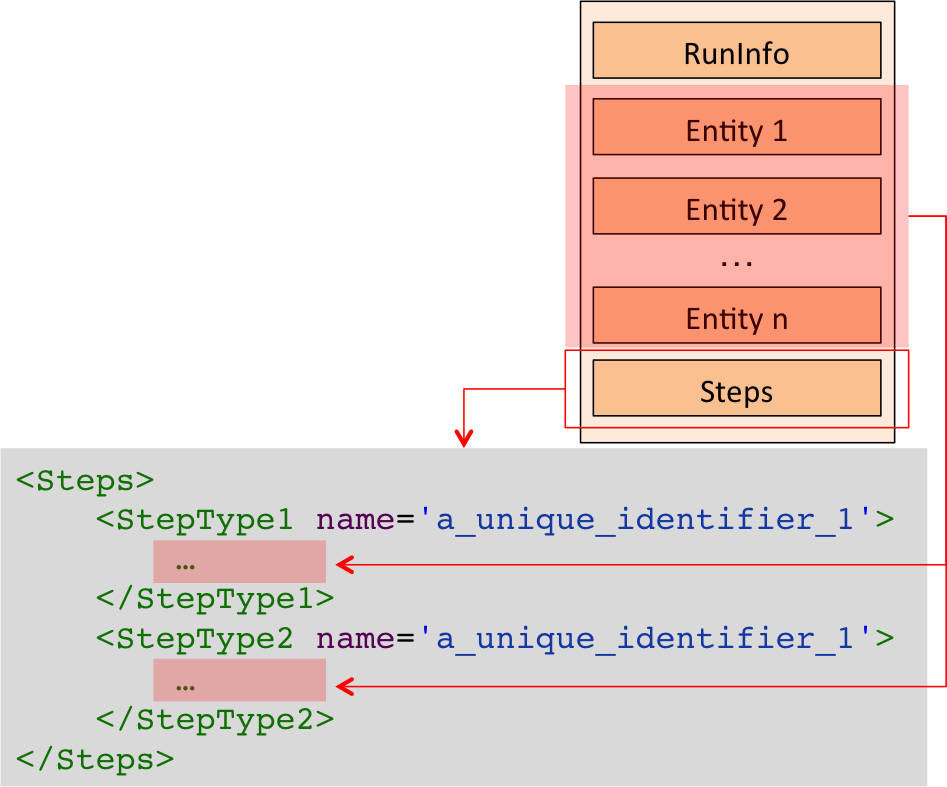
\includegraphics[scale=1]{pics/ExampleStepEntity.png}
  \caption{Example of the Steps \textbf{Entity}  and its connection in the input file.}
  \label{fig:ExampleStepEntity}
\end{figure}

%%%%%%%%%%%%%%%%%%%%%%%%%%%%%%%%%%%%%%%%%%%%%%%%%%%%%%%%%%%%%%%%%
%%%%%%%%%%%%%%%%%%%%%%%%%%%%%%%%%%%%%%%%%%%%%%%%%%%%%%%%%%%%%%%%%
\subsection{Build RAVEN Input: \xmlNode{IOStep}}
The \xmlNode{IOStep} acts as a "transfer network" among different RAVEN storing or streaming objects. The number
of \xmlNode{Input} and \xmlNode{Output} is unlimited. This \xmlNode{IOStep} assumes one-to-one mapping, i.e. the first
\xmlNode{Input} is going to be used for the first \xmlNode{Output}, etc. \nb If the \xmlNode{Output} nodes are class
\xmlString{OutStreams}, the user does not need to follow this assumption, since \textbf{OutStreams} objects are already
linked to \textbf{DataObjects} in the relative RAVEN input block.
The \textbf{IOStep} can be used to:
\begin{itemize}
  \item construct/update a \textit{Database} from a \textit{DataObjects} object, and vice versa;
  \item construct/update a \textit{DataObject} from a \textit{CSV} file contained in a directory;
  \item construct/update a \textit{Database} or a \textit{DataObjects} object from
    \textit{CSV} files contained in a directory;
  \item stream the content of a \textit{Database} or a \textit{DataObjects} out through an \textbf{OutStream} object;
  \item store/retrieve a \textit{ROM} to/from an external \textit{File} using Pickle module of Python.
\end{itemize}
The last function can be used to create and store mathematical model of fast solution trained to predict a
response of interest of a physical system. This model can be recovered in other simulations or used to evaluate
the response of a physical system in a Python program by the implementing of the Pickle module.

%%%%%%%%%%%%%%%%%%%%%%%%%%%%%%%%%%%%%%%%%%%%%%%%%%%%%%%%%%%%%%%%%
\subsubsection{Perform input/output operations}
In this case, we will use \xmlNode{IOStep} to stream the output data from the \textit{DataObjects} out through the
\textit{OutStreams}. The \xmlNode{IOStep} block is shown as follows:
\xmlExample{framework/user_guide/ravenTutorial/singleRunPlotAndPrint.xml}{Steps}
As shown in the \xmlNode{IOStep}, the input is a history set ``history'' that is previous generated by the \textbf{SingleRun}
step. The data stored in the ``history'' will be printed and plotted via the \textbf{OutStreams}.The data object
``history'' is defined as follows:
\xmlExample{framework/user_guide/ravenTutorial/singleRunPlotAndPrint.xml}{DataObjects}
\nb If a \textit{PointSet} data object is used to collect the temporal output data, only the data from the last time
step will be stored in this data object. As demonstrated in this case, the output csv file with name ``pointValues.csv''
generated through the \textbf{OutStreams} in \textbf{SingleRun} step only contains the data for the last time step.
This file can be found in the working directory specified by sub-node \xmlNode{WorkingDir} under node \xmlNode{RunInfo}.

As mentioned before, \textbf{OutStreams} can be used to plot the data stored in the data objects. The following
input block demonstrates the use of \textbf{OutStreams} for plotting.
\xmlExample{framework/user_guide/ravenTutorial/singleRunPlotAndPrint.xml}{OutStreams}
In this block, both the Out-Stream types are constructed:
\begin{itemize}
  \item \textit{Print}: named ``history'' connected with the \textit{DataObjects} \textbf{Entity} ``history'' (\xmlNode{source})
  When this object get used, all the information contained in the linked  \textit{DataObjects} are going
  to be dumped in CSV files (\xmlNode{type}).
  \item \textit{Plot}: a single \xmlNode{Plot} \textbf{Entity} is defined, containing the line plots of the 4 output variables
  ($A,B,C,D$) in the same figure. This object is going to generate a PNG file in the working directory.
\end{itemize}

%figure history
\begin{figure}[h!]
  \centering
  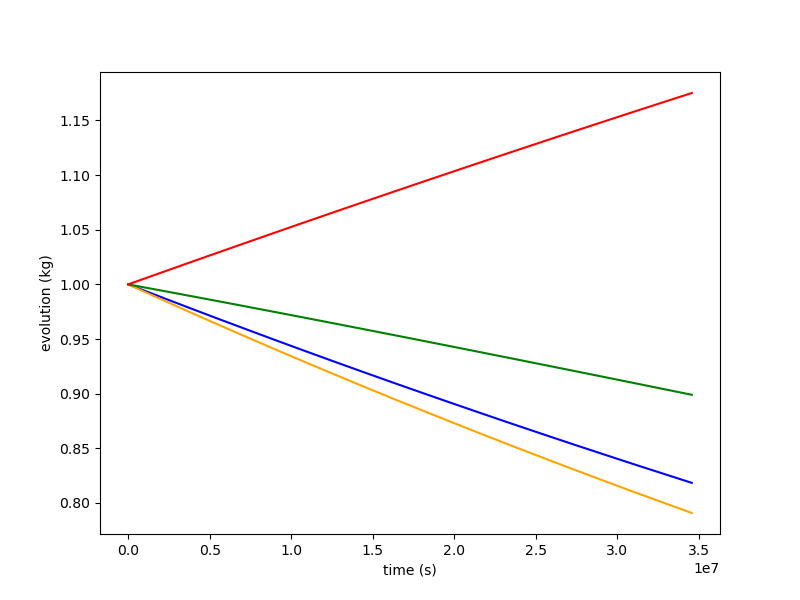
\includegraphics[scale=0.7]{../../tests/framework/user_guide/ravenTutorial/gold/singleRunPlot/1-historyPlot_line-line-line-line.png}
  \caption{Plot of the history for variables $A,B,C,D$.}
  \label{fig:historyPlotLine}
\end{figure}

For examples of the numerical data produced by the OutStreams \textit{Print}, see \texttt{history\_0.csv} in the directory
 \texttt{raven/tests/framework/user\_guide/ravenTutorial/ gold/singleRunPlot/}
 As previously mentioned, Figure~\ref{fig:historyPlotLine} reports the four plots (four variables) drawn in the same picture.

%%%%%%%%%%%%%%%%%%%%%%%%%%%%%%%%%%%%%%%%%%%%%%%%%%%%%%%%%%
%\FloatBarrier
\subsubsection{Sub-plot and selectively printing.}
This section shows how to use RAVEN to create sub-plots (multiple plots in the same figure) and
how to select only some variable from the \textit{DataObjects} in the \textit{Print} OutStream.
 \\ The goals of this Section are about learning how to:
 \begin{enumerate}
   \item Print out what contained in the DataObjects, selecting only few variables
   \item Generate sub-plots (multiple plots in the same figure) of the code results
\end{enumerate}

To accomplish these tasks, the \xmlNode{IOStep} needs to be modified as follows:
\xmlExample{framework/user_guide/ravenTutorial/singleRunSubPlotsAndSelectivePrint.xml}{Steps}
\nb as mentioned before, this \xmlNode{IOStep} does not need to follow the one-to-one mapping, since \textit{OutStreams}
are alreadly linked to the \textit{DataObjects}.
And the \textit{OutStreams} \textbf{Entity} in the input defined in the previous section needs to be modified as
follows:
\xmlExample{framework/user_guide/ravenTutorial/singleRunSubPlotsAndSelectivePrint.xml}{OutStreams}

\begin{enumerate}
   \item \textbf{\textit{Print}}:
   With respect to the \textit{Print} nodes defined in the previous section, it can
   be noticed that an additional node has been added: \xmlNode{what}. The \textit{Print} \textbf{Entity}
   ``pointValues'' is going to extract and dump only the variables that are part of the Output space
   ($A,B,C,D$ and not $InputPlaceHolder$).  The \textit{Print} \textbf{Entity} ``history'' is instead going to print
   the Output space variables $A$ and $D$.

   \item \textbf{\textit{Plot}}:
 Note that the  \textit{Plot} \textbf{Entity} does not differ much with respect to the one in
 previous section: 1) the additional sub-node \xmlNode{gridSpace}  has been added.
 This node is needed to define how the figure needs to be partitioned (discretization of the grid). In this case
 a 2 by 2 grid is requested. 2) in each \xmlNode{plot} the node \xmlNode{gridLocation} is placed in
 order to specify in which position the relative plot needs to be placed. For example, in the following grid
 location, the relative plot is going to be placed at the bottom-right corner.
 \begin{lstlisting}[style=XML,morekeywords={arg,extension,pauseAtEnd,overwrite}]
   <gridLocation>
      <x>1</x>
      <y>1</y>
   </gridLocation>
  \end{lstlisting}
\end{enumerate}

The printed data will dump to the CSV file \textit{history\_0.csv}, and Figure~\ref{fig:historySubPlotLine} reports the four plots (four variables) drawn in the same picture.

%figure history sublots
\begin{figure}[h!]
  \centering
  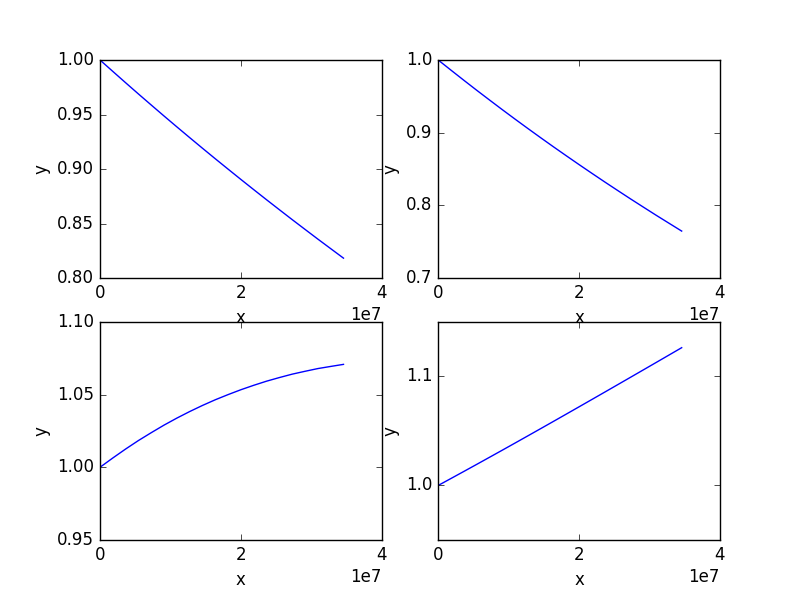
\includegraphics[scale=0.7]{../../tests/framework/user_guide/ravenTutorial/gold/subPlot/1-historyPlot_line-line-line-line.png}
  \caption{Subplot of the history for variables $A,B,C,D$.}
  \label{fig:historySubPlotLine}
\end{figure}

\section{Forward Sampling Strategies}
\label{sec:forwardSamplingStrategies}
In order to perform UQ and dynamic
probabilistic risk assessment (DPRA),
a sampling strategy needs to be employed. The sampling strategy
perturbs the input space (domain of the uncertainties) to explore
the response of a complex system in relation to selected FOMs.

The most widely used strategies to perform UQ and PRA are generally
collected in RAVEN as \textit{\textbf{Forward}} samplers. \textit{\textbf{Forward}} samplers include
all the strategies that simply perform the sampling of the input space.  These strategies sample
without exploiting, through learning approaches,
the information made available from the outcomes of evaluation previously performed (adaptive sampling) and the
common system evolution (patterns) that different sampled calculations can generate in the phase space (Dynamic Event Tree).

As mentioned in Section~\ref{sub:tutorialMultiRun}, RAVEN has
several different \textit{\textbf{Forward}} samplers:
\begin{itemize}
  \item \textit{Monte-Carlo}
  \item \textit{Grid-based}
  \item \textit{Stratified} and its specialization named \textit{Latin Hyper Cube}.
\end{itemize}
In addition, RAVEN posses advanced \textit{\textbf{Forward}} sampling strategies that:
\begin{itemize}
  \item Build a grid in the input space selecting evaluation points
    based on characteristic quadratures as part of stochastic collocation
    for generalized polynomial chaos method (\textit{Sparse
    Grid Collocation} sampler);
  \item Use high-density model reduction (HDMR) a.k.a. Sobol
    decomposition to approximate a function as the sum of
    interactions with increasing complexity (\textit{Sobol} sampler).
\end{itemize}
In the following subsections, we provide examples of input files
in RAVEN using the method, with explanatory commentary.
%%%%%%%%%%%%%%%%%%%%%%%%%
%%%%%%%%  MONTE-CARLO %%%%%%%%
%%%%%%%%%%%%%%%%%%%%%%%%%
\subsection{Monte-Carlo sampling through RAVEN}
\label{sub:MCexample}
The Monte-Carlo method is one of the most-used methodologies in several mathematic disciplines. In this section,
we will explain the techniques for employing this methodology in RAVEN, and we recommend the user to read the
theory manual to explore the theory of the method.
The goals of this section are about learning how to:
 \begin{enumerate}
   \item Set up a simple Monte-Carlo sampling for perturbing the input space of a driven code
   \item Load the outputs of the code into RAVEN DataObjects (HistorySets and PointSets)
   \item Print the contents of DataObjects to file
   \item Generate plots of the sampling results.
\end{enumerate}
In order to accomplish these tasks, the following RAVEN \textbf{Entities} (XML blocks in the RAVEN input file) are needed:
\begin{enumerate}
   \item \textbf{\textit{RunInfo}}:
     \xmlExample{framework/user_guide/ForwardSamplingStrategies/forwardSamplingMontecarlo.xml}{RunInfo}
     As discussed in Section~\ref{sub:singleRun}, the \textit{RunInfo} \textbf{Entity} sets up the analysis
     that the user wants to perform. The number of steps specified in (\xmlNode{Sequence}) are sequentially run using the number of processors assigned in (\xmlNode{batchSize}). 
     Note that the \xmlNode{JobName} is not required, but is useful in identifying the input file.
   \item \textbf{\textit{Models}}:
     \xmlExample{framework/user_guide/ForwardSamplingStrategies/forwardSamplingMontecarlo.xml}{Models}
     The Model used in this example is the \textbf{Projectile} external model, which is defined in section \ref{sec:analyticalbateman}.  
   \item \textbf{\textit{Distributions}}:
     \xmlExample{framework/user_guide/ForwardSamplingStrategies/forwardSamplingMontecarlo.xml}{Distributions}
     In the \xmlNode{Distributions} block, the stochastic model for the uncertainties treated by the
     \xmlNode{Sampler} is defined. In this case two distributions are defined:
  \begin{itemize}
    \item $vel\_dist \sim \mathbb{N}(30,5)$, used to model the uncertainties
    associated with  the \textit{velocity};
    \item  $angle\_dist \sim \mathbb{U}(5,85)$,  used to
    model the uncertainties associated with the \textit{angle}.
  \end{itemize}
   \item \textbf{\textit{Samplers}}:
     \xmlExample{framework/user_guide/ForwardSamplingStrategies/forwardSamplingMontecarlo.xml}{Samplers}
      To employ the Monte-Carlo sampling strategy, a
      \xmlNode{MonteCarlo} node needs to be defined. The number of samples is defined within this node. The Monte-Carlo method is employed on model variables listed by name and are associated with a distribution.
   \item \textbf{\textit{DataObjects}}:
     \xmlExample{framework/user_guide/ForwardSamplingStrategies/forwardSamplingMontecarlo.xml}{DataObjects}
      In this block, three \textit{DataObjects} are defined to store results: 1) a PointSet named
      ``samples'', 2) a PointSet named ``dummyIN'' 3) a HistorySet named ``histories''.
      Note that in the \xmlNode{Input} node all the uncertainties
      perturbed through the Monte-Carlo strategy are listed. By this, any
      realization in the input space is linked in the DataObject to the outputs listed in the
      \xmlNode{Output} node. Furthermore, since we use an external model that does not have any input file, we define a pointset named ``dummyIN'' that is used as a dummy input in the multirun step.
   \item \textbf{\textit{OutStreams}}:
     \xmlExample{framework/user_guide/ForwardSamplingStrategies/forwardSamplingMontecarlo.xml}{OutStreams}
 %%%%%%%%%%%%%%%%%%%%%%%%%%%%%%%%%%%%%%%%%%%%%%%%%%%%%%%%%%
 %figure histories
 \begin{figure}[h!]
  \centering
  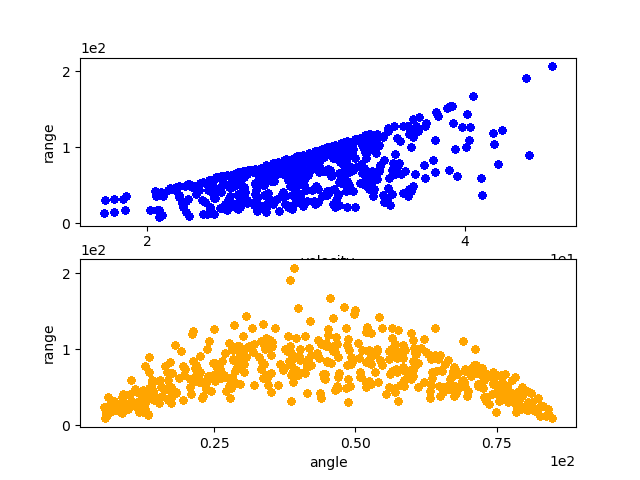
\includegraphics[scale=0.7]{../../tests/framework/user_guide/ForwardSamplingStrategies/gold/RunDir/MonteCarlo/1-historyPlot_scatter-scatter.png}
  \caption{Plot of the histories generated by the Monte Carlo sampling.}
  \label{fig:historiesMCPlotScatter}
 \end{figure}
 %%%%%%%%%%%%%%%%%%%%%%%%%%%%%%%%%%%%%%%%%%%%%%%%%%%%%%%%%%
 To see the results of the simulation, \xmlNode{OutStreams} are included in the input.
  In this block, both OutStream types are used:
  \begin{itemize}
    \item \textit{Print}:
     \begin{itemize}
       \item ``samples'' connected with the \textit{DataObjects} \textbf{Entity} ``samples''
                (\xmlNode{source})
       \item ``histories'' connected with the \textit{DataObjects} \textbf{Entity} ``histories'' (\xmlNode{source})
     \end{itemize}
     Note that in RAVEN, multiple entities can have the same name, as it takes a class, a type, and a name to uniquely identify a RAVEN object. When the two OutStream objects are used, all the information contained in the  linked \textit{DataObjects} are going
    to be exported in CSV files (\xmlNode{type}).
    \item \textit{Plot}:
    \begin{itemize}
      \item ``historiesPlot'' connected with the  \textit{DataObjects}
      \textbf{Entity} ``histories''.  This plot shows the variable $range$ with respect to the input variables $velocity$ and $angle$.
      \item ``samplesPlot3D'' connected with the
      \textit{DataObjects} \textbf{Entity} ``samples''. This plot shows the variables $range,time$ with respect to the input variables $velocity$ and $angle$.
    \end{itemize}
     Note that both plots use gridded subplots. Two plots
     are placed in each of the figures.
  \end{itemize}
   \item \textbf{\textit{Steps}}:
     \xmlExample{framework/user_guide/ForwardSamplingStrategies/forwardSamplingMontecarlo.xml}{Steps}
 %%%%%%%%%%%%%%%%%%%%%%%%%%%%%%%%%%%%%%%%%%%%%%%%%%%%%%%%%%
 %figure samples
 \begin{figure}[h!]
  \centering
  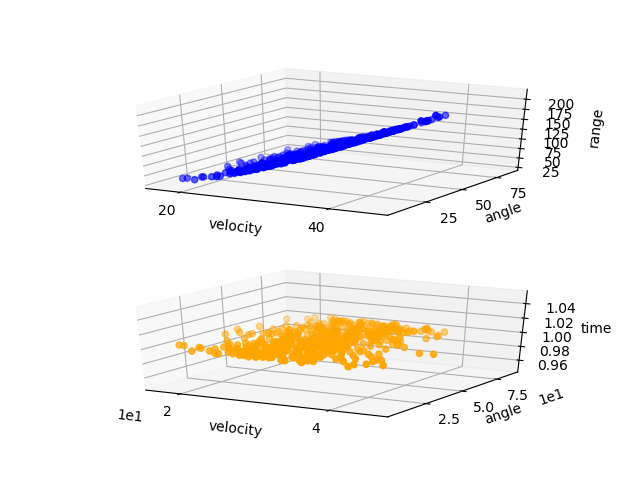
\includegraphics[scale=0.7]{../../tests/framework/user_guide/ForwardSamplingStrategies/gold/RunDir/MonteCarlo/1-samplesPlot3D_scatter-scatter.png}
  \caption{Plot of the samples generated by the MC sampling.}
  \label{fig:samplesMCPlotScatter}
 \end{figure}
 %%%%%%%%%%%%%%%%%%%%%%%%%%%%%%%%%%%%%%%%%%%%%%%%%%%%%%%%%%
   Once all the other entities are defined in the RAVEN input file, they must be combined in the
   \xmlNode{Steps} block, which dictates the workflow of RAVEN.  For this case,
   two \xmlNode{Steps} are defined:
   \begin{itemize}
     \item \xmlNode{MultiRun} ``sample'', used to run the multiple
     instances of the driven code and
     collect the outputs in the two \textit{DataObjects}. As it can be
     seen, the \xmlNode{Sampler} is specified to communicate to the
     \textit{Step} that the driven code needs to
     be perturbed through the Monte-Carlo sampling.
     \item  \xmlNode{IOStep} named ``writeHistories'', used to 1) dump
     the ``histories'' and ``samples'' \textit{DataObjects}
     \textbf{Entity} to a CSV file and 2) plot the data in the EPS file.
   \end{itemize}
\end{enumerate}
 Figures~\ref{fig:historiesMCPlotScatter} and ~\ref{fig:samplesMCPlotScatter} show the report
 generated by RAVEN.
%%%%%%%%%%%%%%%%%%%%%%%%%
%%%%%%%%          GRID          %%%%%%%%
%%%%%%%%%%%%%%%%%%%%%%%%%
\subsection{Grid sampling through RAVEN}
\label{sub:Gridexample}
The Grid sampling method (also known as Full Factorial Design of Experiment) represents one of the simplest methodologies that can be employed in order to explore the interaction of multiple random variables with respect
selected FOMs.
The goal of this section is to show how to:
 \begin{enumerate}
   \item Set up a simple Grid sampling for performing a parametric analysis of a driven code
   \item Load the outputs of the code into the RAVEN DataObjects system
   \item Print out what contained in the DataObjects
   \item Generate basic plots of the code result.
\end{enumerate}
In order to accomplish these tasks, the following RAVEN \textbf{Entities} (XML blocks in the input files) are required:
\begin{enumerate}
   \item \textbf{\textit{RunInfo}}:
     \xmlExample{framework/user_guide/ForwardSamplingStrategies/forwardSamplingGrid.xml}{RunInfo}
   As shown in Section~\ref{sub:singleRun}, the \textit{RunInfo} \textbf{Entity} is intended to set up the desired analysis. The number of steps specified in (\xmlNode{Sequence}) are sequentially run using the number of processors assigned in (\xmlNode{batchSize}). 
   \item \textbf{\textit{Models}}:
     \xmlExample{framework/user_guide/ForwardSamplingStrategies/forwardSamplingGrid.xml}{Models}
 The Model here is represented by the \textbf{Projectile}, which already dumps its output file in a
 CSV format (standard format that RAVEN can read). 
   \item \textbf{\textit{Distributions}}:
     \xmlExample{framework/user_guide/ForwardSamplingStrategies/forwardSamplingGrid.xml}{Distributions}
  In the Distributions XML section, the stochastic model for the
  uncertainties  treated by the Grid sampling are reported. In
  this case two distributions are defined:
  \begin{itemize}
    \item $vel\_dist \sim \mathbb{N}(30,5)$, used to model the uncertainties
    associated with  the \textit{velocity};
    \item  $angle\_dist \sim \mathbb{U}(5,85)$,  used to
    model the uncertainties associated with the \textit{angle}.
  \end{itemize}
   \item \textbf{\textit{Samplers}}:
     \xmlExample{framework/user_guide/ForwardSamplingStrategies/forwardSamplingGrid.xml}{Samplers}
  To employ the Grid sampling strategy, a
  \xmlNode{Grid} node needs to be specified. As shown above, in each variable section, the  \xmlNode{grid} is defined.
   \item \textbf{\textit{DataObjects}}:
     \xmlExample{framework/user_guide/ForwardSamplingStrategies/forwardSamplingGrid.xml}{DataObjects}
  In this block, three \textit{DataObjects} are defined to store results: 1) a PointSet named
      ``samples'', 2) a PointSet named ``dummyIN'' 3) a HistorySet named ``histories''.
  In the \xmlNode{Input} node all the variables  perturbed through the Grid strategy are listed. In this way, any  realization in the input space is linked to the outputs listed in  the
  \xmlNode{Output} node. As described earlier as well, since we use an external model that does not have any input file, we define a pointset named ``dummyIN'' that is used as a dummy input in the multirun step.
    \item \textbf{\textit{OutStreams}}:
     \xmlExample{framework/user_guide/ForwardSamplingStrategies/forwardSamplingGrid.xml}{OutStreams}
 %%%%%%%%%%%%%%%%%%%%%%%%%%%%%%%%%%%%%%%%%%%%%%%%%%%%%%%%%%
 %figure histories
 \begin{figure}[h!]
  \centering
  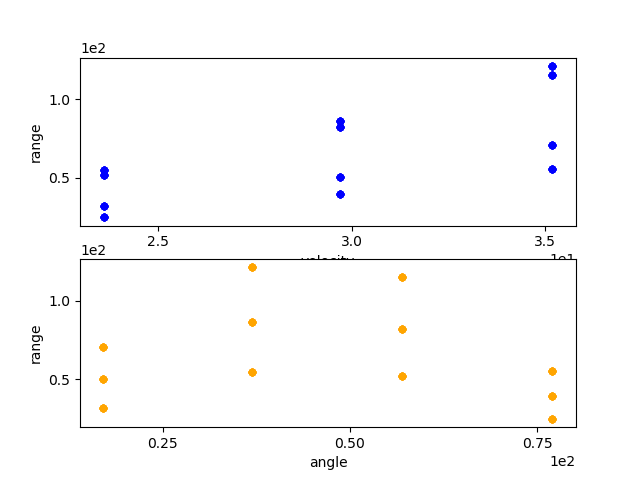
\includegraphics[scale=0.7]{../../tests/framework/user_guide/ForwardSamplingStrategies/gold/RunDir/Grid/1-historyPlot_scatter-scatter.png}
  \caption{Plot of the histories generated by the Grid sampling.}
  \label{fig:historiesGridPlotScatter}
 \end{figure}
 %%%%%%%%%%%%%%%%%%%%%%%%%%%%%%%%%%%%%%%%%%%%%%%%%%%%%%%%%%
  In this block, both the Out-Stream types are constructed:
  \begin{itemize}
    \item \textit{Print}:
     \begin{itemize}
       \item named ``samples'' connected with the \textit{DataObjects} \textbf{Entity} ``samples''
                (\xmlNode{source})
       \item named ``histories'' connected with the \textit{DataObjects} \textbf{Entity} ``histories'' (\xmlNode{source}).
     \end{itemize}
      When these objects get used, all the information contained in the
      linked  \textit{DataObjects} are going
    to be exported in CSV files (\xmlNode{type}).
    \item \textit{Plot}:
    \begin{itemize}
      \item named ``historiesPlot'' connected with the  \textit{DataObjects}
      \textbf{Entity} ``histories''.  This plot shows the variable $range$ with respect to the input variables $velocity$ and $angle$.
      \item named ``samplesPlot3D'' connected with the
      \textit{DataObjects} \textbf{Entity} ``samples''. This plot shows the variables $range,time$ with respect to the input variables $velocity$ and $angle$.
    \end{itemize}
  \end{itemize}
   \item \textbf{\textit{Steps}}:
     \xmlExample{framework/user_guide/ForwardSamplingStrategies/forwardSamplingGrid.xml}{Steps}
 %%%%%%%%%%%%%%%%%%%%%%%%%%%%%%%%%%%%%%%%%%%%%%%%%%%%%%%%%%
 %figure samples
 \begin{figure}[h!]
  \centering
  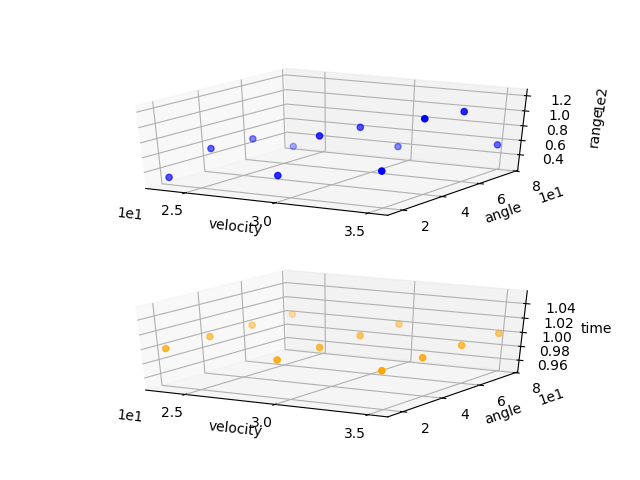
\includegraphics[scale=0.7]{../../tests/framework/user_guide/ForwardSamplingStrategies/gold/RunDir/Grid/1-samplesPlot3D_scatter-scatter.png}
  \caption{Plot of the samples generated by the Grid sampling for variables $A,B,C,D$.}
  \label{fig:samplesGridPlotScatter}
 \end{figure}
 %%%%%%%%%%%%%%%%%%%%%%%%%%%%%%%%%%%%%%%%%%%%%%%%%%%%%%%%%%
   Finally, all the previously defined \textbf{Entities} can be combined in
   the \xmlNode{Steps} block. As inferable,
   two \xmlNode{Steps} have been inputted:
   \begin{itemize}
     \item \xmlNode{MultiRun} named ``sample'', is used to run the multiple
     instances of the code and
     collect the outputs in the two \textit{DataObjects}. As it can be
     seen, the \xmlNode{Sampler} is inputted to communicate to the
     \textit{Step} that the driven code needs to
     be perturbed through the Grid sampling
     \item  \xmlNode{IOStep} named ``writeHistories'', used to 1) dump
     the ``histories'' and ``samples'' \textit{DataObjects}
     \textbf{Entity} in a CSV file and 2) plot the data in the PNG file and
     on the screen.
   \end{itemize}
\end{enumerate}
 Figures~\ref{fig:historiesGridPlotScatter} and ~\ref{fig:samplesGridPlotScatter} display the report generated by RAVEN.

%%%%%%%%%%%%%%%%%%%%%%%%%
%%%%%%%%    STRATIFIED    %%%%%%%%
%%%%%%%%%%%%%%%%%%%%%%%%%
\subsection{Stratified sampling through RAVEN}
\label{sub:Stratifiedexample}
The Stratified sampling is a class of methods that relies on the assumption that the input space (i.e.,uncertainties)
can be separated in regions (strata) based on similarity of the response of the system for input set within the
same strata. Following this assumption, the most rewarding (in terms of computational cost vs. knowledge gain)
sampling strategy would be to place one sample for each region. In this way, the same information is not
collected more than once and all the prototypical behavior are sampled at least once. In
Figure~\ref{fig:StratifiedSamplingExample}, the Stratified sampling approach is exemplified.
 \begin{figure}[h!]
  \centering
  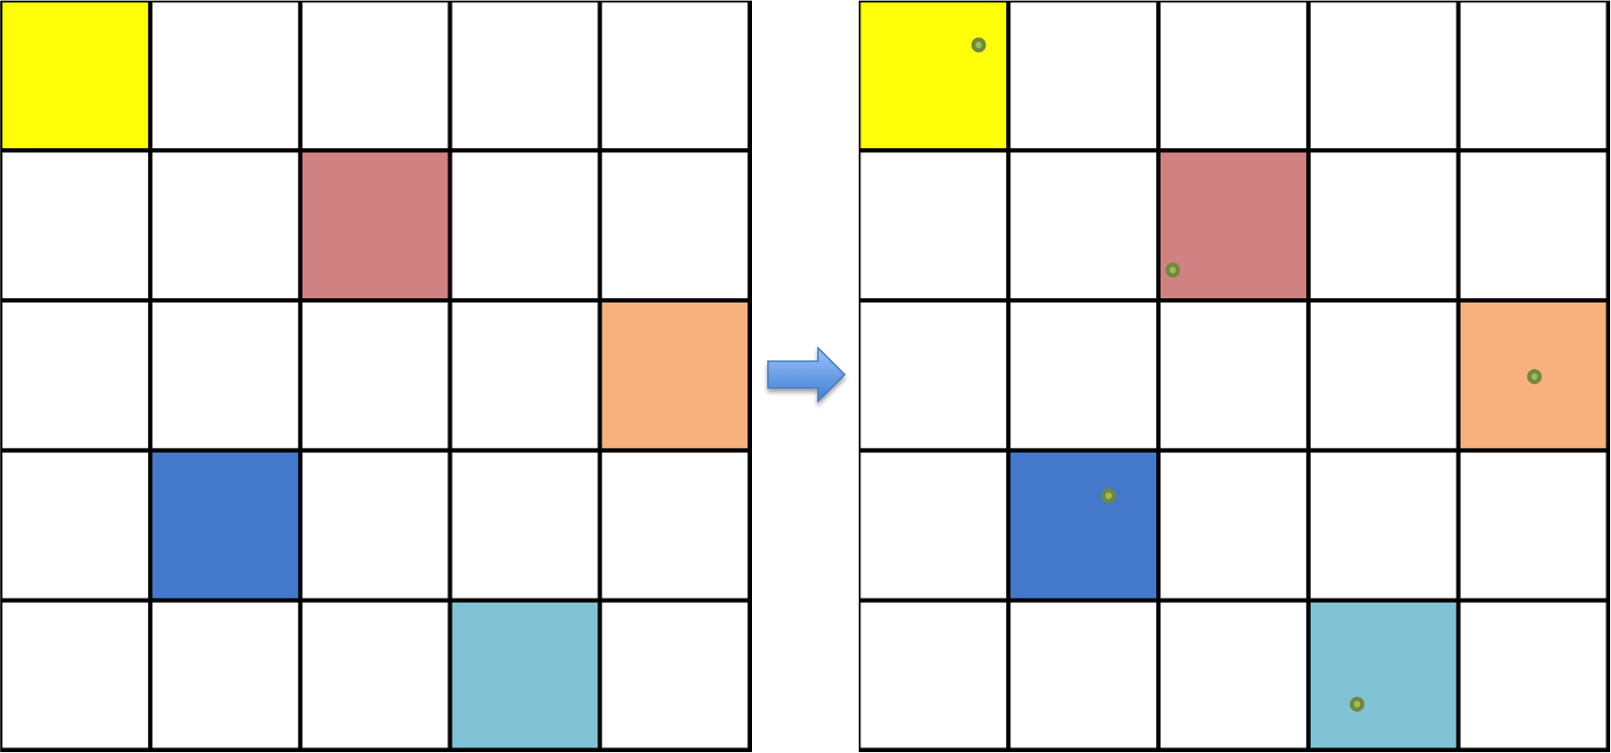
\includegraphics[scale=0.55]{pics/StratifiedSamplingExample.png}
  \caption{Example of Stratified sampling approach.}
  \label{fig:StratifiedSamplingExample}
 \end{figure}
\\The goal of this section is to show how to:
 \begin{enumerate}
   \item Set up a simple Stratified sampling in order to perform a parametric analysis on a driven code
   \item Load the outputs of the code into the RAVEN DataObjects system
   \item Print out what contained in the DataObjects
   \item Generate basic plots of the code result.
\end{enumerate}
To accomplish these tasks, the following RAVEN \textbf{Entities} (XML blocks in the input files) are defined:
\begin{enumerate}
   \item \textbf{\textit{RunInfo}}:
     \xmlExample{framework/user_guide/ForwardSamplingStrategies/forwardSamplingStratified.xml}{RunInfo}
   As explained earlier, the \textit{RunInfo} \textbf{Entity} is intended to set up the analysis that the user wants to perform. The number of steps specified in (\xmlNode{Sequence}) are sequentially run using the number of processors assigned in (\xmlNode{batchSize}).
   \item \textbf{\textit{Models}}:
     \xmlExample{framework/user_guide/ForwardSamplingStrategies/forwardSamplingStratified.xml}{Models}
 The Model here is represented by the
 \textbf{Projectile}, which already dumps its output file in a
 CSV format (standard format that RAVEN can read).
   \item \textbf{\textit{Distributions}}:
     \xmlExample{framework/user_guide/ForwardSamplingStrategies/forwardSamplingStratified.xml}{Distributions}
  In the Distributions XML section, the stochastic model for the
  uncertainties  treated by the Stratified sampling are reported. In
  this case two distributions are defined:
  \begin{itemize}
    \item $vel\_dist \sim \mathbb{N}(30,5)$, used to model the uncertainties
    associated with  the \textit{velocity};
    \item  $angle\_dist \sim \mathbb{U}(5,85)$,  used to
    model the uncertainties associated with the \textit{angle}.
  \end{itemize}
   \item \textbf{\textit{Samplers}}:
     \xmlExample{framework/user_guide/ForwardSamplingStrategies/forwardSamplingStratified.xml}{Samplers}
  To employ the Stratified sampling strategy, a
  \xmlNode{Stratified} node needs to be specified. In each variable section, the  \xmlNode{grid} is defined.
  It is important to mention that the number of \xmlAttr{steps} needs to be the same for each of the variables,  since, as reported in previous section, the Stratified sampling strategy it discretizes the domain in strata.
  The number of samples finally requested is equal to $n_{samples} = n_{steps} = 100$.
  If the grid for each variables is defined in CDF and of  \xmlAttr{type} = ``equal'', the Stratified sampling corresponds to the well-known Latin Hyper Cube sampling.
   \item \textbf{\textit{DataObjects}}:
     \xmlExample{framework/user_guide/ForwardSamplingStrategies/forwardSamplingStratified.xml}{DataObjects}
  In this block, two \textit{DataObjects} are defined: 1) a PointSet named
      ``samples'', 2) a PointSet named ``dummyIN'' 3) a HistorySet named ``histories''.
  In the \xmlNode{Input} node all the variables perturbed through the Stratified strategy are listed. In this way, any realization in the input space is linked to the outputs listed in  the
  \xmlNode{Output} node. Since we use an external model that does not have any input file, we define a pointset named ``dummyIN'' that is used as a dummy input in the multirun step.
   \item \textbf{\textit{OutStreams}}:
     \xmlExample{framework/user_guide/ForwardSamplingStrategies/forwardSamplingStratified.xml}{OutStreams}
 %%%%%%%%%%%%%%%%%%%%%%%%%%%%%%%%%%%%%%%%%%%%%%%%%%%%%%%%%%
 %figure histories
 \begin{figure}[h!]
  \centering
  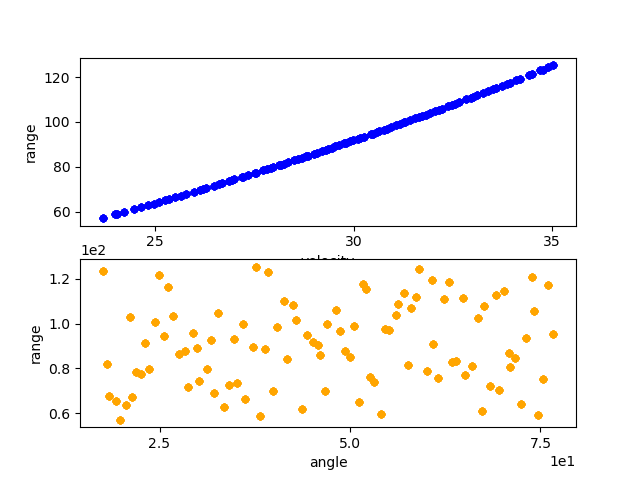
\includegraphics[scale=0.7]{../../tests/framework/user_guide/ForwardSamplingStrategies/gold/RunDir/Stratified/1-historyPlot_scatter-scatter.png}
  \caption{Plot of the histories generated by the Stratified sampling.}
  \label{fig:historiesStratifiedPlotScatter}
 \end{figure}
 %%%%%%%%%%%%%%%%%%%%%%%%%%%%%%%%%%%%%%%%%%%%%%%%%%%%%%%%%%
  In this block, both the Out-Stream types are constructed:
  \begin{itemize}
    \item \textit{Print}:
     \begin{itemize}
       \item named ``samples'' connected with the \textit{DataObjects} \textbf{Entity} ``samples''
                (\xmlNode{source})
       \item named ``histories'' connected with the \textit{DataObjects} \textbf{Entity} ``histories'' (\xmlNode{source}).
     \end{itemize}
      When these objects get used, all the information contained in the
      linked  \textit{DataObjects} are going
    to be exported in CSV files (\xmlNode{type}).
    \item \textit{Plot}:
    \begin{itemize}
      \item named ``historiesPlot'' connected with the  \textit{DataObjects}
      \textbf{Entity} ``histories''.  This plot shows the variable $range$ with respect to the input variables $velocity$ and $angle$.
      \item named ``samplesPlot3D'' connected with the
      \textit{DataObjects} \textbf{Entity} ``samples''. This plot shows the variables $range,time$ with respect to the input variables $velocity$ and $angle$.
    \end{itemize}
  \end{itemize}
   \item \textbf{\textit{Steps}}:
     \xmlExample{framework/user_guide/ForwardSamplingStrategies/forwardSamplingStratified.xml}{Steps}
 %%%%%%%%%%%%%%%%%%%%%%%%%%%%%%%%%%%%%%%%%%%%%%%%%%%%%%%%%%
 %figure samples
 \begin{figure}[h!]
  \centering
  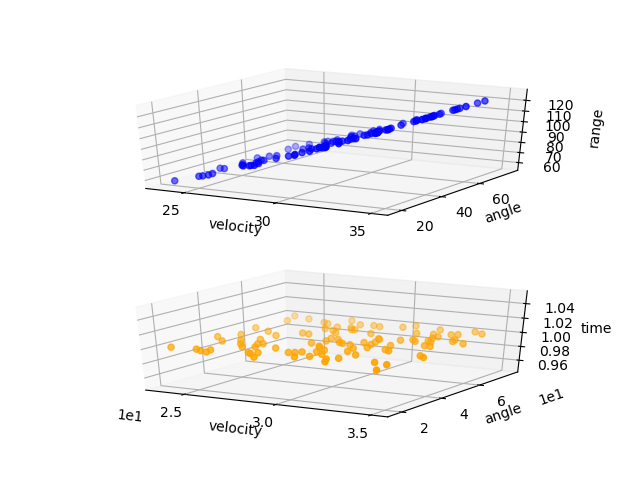
\includegraphics[scale=0.7]{../../tests/framework/user_guide/ForwardSamplingStrategies/gold/RunDir/Stratified/1-samplesPlot3D_scatter-scatter.png}
  \caption{Plot of the samples generated by the Stratified sampling.}
  \label{fig:samplesStratifiedPlotLine}
 \end{figure}
 %%%%%%%%%%%%%%%%%%%%%%%%%%%%%%%%%%%%%%%%%%%%%%%%%%%%%%%%%%
   Finally, all the previously defined \textbf{Entities} can be combined in
   the \xmlNode{Steps} block. As inferable,
   two \xmlNode{Steps} have been inputted:
   \begin{itemize}
     \item \xmlNode{MultiRun} named ``sample'', used to run the multiple
     instances of the driven code and
     collect the outputs in the two \textit{DataObjects}. As it can be
     seen, the \xmlNode{Sampler} is inputted to communicate to the
     \textit{Step} that the driven code needs to
     be perturbed through the Stratified sampling.
     \item  \xmlNode{IOStep} named ``writeHistories'', used to 1) dump
     the ``histories'' and ``samples'' \textit{DataObjects}
     \textbf{Entity} in a CSV file and 2) plot the data in the PNG file and
     on the screen.
   \end{itemize}
\end{enumerate}
 As previously mentioned, Figures~\ref{fig:historiesStratifiedPlotScatter} and ~\ref{fig:samplesStratifiedPlotScatter}  display the report generated by RAVEN.

%%%%%%%%%%%%%%%%%%%%%%%%%

\subsection{Sparse Grid Collocation sampling through RAVEN}
\label{sub:SGcsamplingExample}
The Sparse Grid Collocation sampler represents an advanced methodology to perform Uncertainty Quantification. They aim
to explore the input space leveraging the information contained in the associated probability density functions. It builds on generic Grid sampling by selecting evaluation points based on characteristic quadratures as part of stochastic collocation for generalized polynomial chaos uncertainty quantification. In collocation an N-D grid is constructed, with each uncertain variable providing an axis. Along each axis, the points of evaluation correspond to quadrature points necessary to integrate polynomials. In the simplest (and most naive) case, a N-D tensor product of all possible combinations of points from each dimension’s quadrature is constructed as sampling points. The number of necessary samples can be reduced by employing Smolyak-like sparse grid algorithms, which use reduced combinations of polynomial orders to reduce the necessary sampling space.
\\The goals of this section are about learning how to:
 \begin{enumerate}
   \item Set up a Sparse Grid Collocation sampling for the construction of a suitable surrogate model of a driven code
   \item Construct a GaussPolynomialRom surrogate model (training stage)
   \item Use the constructed GaussPolynomialRom surrogate model instead of the driven code.
\end{enumerate}
To accomplish these tasks, the following RAVEN \textbf{Entities} (XML blocks in the input files) need to be defined:
\begin{enumerate}
   \item \textbf{\textit{RunInfo}}:
     \xmlExample{framework/user_guide/ForwardSamplingStrategies/forwardSamplingSparseGrid.xml}{RunInfo}
   AThe \textit{RunInfo} \textbf{Entity} is intended to set up the analysis  that the user wants to perform. The steps listed in (\xmlNode{Sequence}) are going to be sequentially run using the number of processors specified in  (\xmlNode{batchSize}).  The first two steps build the ROM
   (\xmlString{sample}, \xmlString{train}), the next two validate
   the ROM against the original Code Model (\xmlString{validateModel}, \xmlString{validateROM}),
   \xmlString{rom\_stats} stores ROM-related information into DataObject,
   and the last two produce plots and print data (\xmlString{output\_print}, \xmlString{output\_plot}).
   \item \textbf{\textit{Models}}:
     \xmlExample{framework/user_guide/ForwardSamplingStrategies/forwardSamplingSparseGrid.xml}{Models}
 The goal of this example is the generation of a \text{GaussPolynomialRom}
 for subsequent usage.  In addition to the previously explained External model, the ROM of type \textit{GaussPolynomialRom} is specified here. The ROM is generated through a Sparse Grid Collocation sampling strategy. Note that the \xmlNode{Interpolation} nodes are not required, but are included for the sake of demonstration.
   \item \textbf{\textit{Distributions}}:
     \xmlExample{framework/user_guide/ForwardSamplingStrategies/forwardSamplingSparseGrid.xml}{Distributions}
  In the Distributions XML section, the stochastic model for the
  uncertainties  treated by the Sparse Grid Collocation sampling are reported. In
  this case two distributions are defined:
  \begin{itemize}
    \item $vel\_dist \sim \mathbb{N}(30,5)$, used to model the uncertainties
    associated with  the \textit{velocity};
    \item  $angle\_dist \sim \mathbb{U}(5,85)$,  used to
    model the uncertainties associated with the \textit{angle}.
  \end{itemize}
   \item \textbf{\textit{Samplers}}:
     \xmlExample[rom,ROM,SparseGridCollocation,MonteCarlo]{framework/user_guide/ForwardSamplingStrategies/forwardSamplingSparseGrid.xml}{Samplers}
  In order to employ the Sparse Grid Collocation sampling strategy, a
  \xmlNode{SparseGridCollocation} node needs to be defined.
  As can be  seen from above, each variable is associated with a different distribution,
  defined in the  \xmlNode{Distributions} block.
  In addition, the \textit{GaussPolynomialRom} \xmlNode{ROM} is linked to the \xmlNode{SparseGridCollocation} sampler.  Because this sampler is used exclusively to build the ROM, some of the parameters of the ROM are  needed by the sampler, and this connection makes that communication possible.  The setting of this ROM (e.g. polynomial order, Index set method, etc.) determines how the Stochastic Collocation Method is employed.

  Additionally, a \xmlNode{MonteCarlo} sampler is set up for validating the ROM against the original Code.  The random number generation seed (\xmlNode{initialSeed}) is specified and set to reset on each use (\xmlNode{reseedEachIteration}) so that the Monte Carlo sampler can be used to compare the ROM against the  original model.  We use 100 samples (\xmlNode{limit}) to sample the ROM and the model, and then print and plot both data sets to compare them.
   \item \textbf{\textit{DataObjects}}:
     \xmlExample[rom,SparseGridCollocation]{framework/user_guide/ForwardSamplingStrategies/forwardSamplingSparseGrid.xml}{DataObjects}
  In this block, five \textit{DataObjects} are defined:
  1) a PointSet named ``inputPlaceholder'' used as a placeholder input for the ROM sampling step,
  2) a PointSet named ``samplesModel'' to store the Code responses from Monte Carlo samples,
  3) a PointSet named ``samplesROM'' to store the ROM responses from Monte Carlo samples,
  4) a HistorySet named ``histories'' used to collect the samples needed to train the ROM, and
  5) a DataSet named ``rom\_stats'' to store information from the ROM.
 %%%%%%%%%%%%%%%%%%%%%%%%%%%%%%%%%%%%%%%%%%%%%%%%%%%%%%%%%%
 %%%%%%%%%%%%%%%%%%%%%%%%%%%%%%%%%%%%%%%%%%%%%%%%%%%%%%%%%%
 %figure histories
 \begin{figure}[h!]
  \centering
  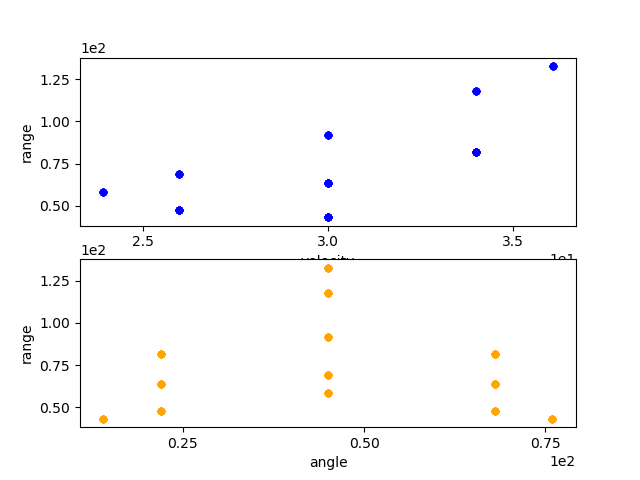
\includegraphics[scale=0.7]{../../tests/framework/user_guide/ForwardSamplingStrategies/gold/RunDir/SparseGrid/1-historyPlot_scatter-scatter.png}
  \caption{Plot of the training samples generated by the SparseGridCollocation sampling for variables $A,B,C,D$.}
  \label{fig:historiesSparseGridPlotScatter}
 \end{figure}
 %%%%%%%%%%%%%%%%%%%%%%%%%%%%%%%%%%%%%%%%%%%%%%%%%%%%%%%%%%
 %%%%%%%%%%%%%%%%%%%%%%%%%%%%%%%%%%%%%%%%%%%%%%%%%%%%%%%%%%
   \item \textbf{\textit{OutStreams}}:
     \xmlExample{framework/user_guide/ForwardSamplingStrategies/forwardSamplingSparseGrid.xml}{OutStreams}
  In this block, the following Out-Stream types are constructed:
  \begin{itemize}
    \item \textit{Print}:
     \begin{itemize}
       \item named ``samplesModel'' connected with the \textit{DataObjects} \textbf{Entity} ``samplesModel''
                (\xmlNode{source})
       \item named ``samplesROM'' connected with the \textit{DataObjects} \textbf{Entity} ``samplesROM''
                (\xmlNode{source})
       \item named ``histories'' connected with the \textit{DataObjects} \textbf{Entity} ``histories'' (\xmlNode{source})
       \item named ``rom\_output'' connected with the \textit{ROM} \textbf{Entity} ``rom'' (\xmlNode{source}).
     \end{itemize}
      When these objects get used, all the information contained in the
      linked  \textit{DataObjects} are going
    to be exported in ether CSV files for DataObjects or XML files for ROMs (\xmlNode{type}).
    \item \textit{Plot}:
    \begin{itemize}
      \item named ``historyPlot'' connected with the  \textit{DataObjects}
      \textbf{Entity} ``histories''.  This plots the
      variable $range$ with respect to the input variables $velocity$ and $angle$.
      \item named ``samplesModelPlot3D'' connected with the
      \textit{DataObjects} \textbf{Entity} ``samplesModel''. This plot will draw the
      variables $range,time$ as Monte Carlo sampled on the Code.
      \item named ``samplesROMPlot3D'' connected with the
      \textit{DataObjects} \textbf{Entity} ``samplesROM''. This plot will draw the
      variables $range,time$ as Monte Carlo sampled on the ROM.
    \end{itemize}
  \end{itemize}
   \item \textbf{\textit{Steps}}:
     \xmlExample[rom,SparseGridCollocation]{framework/user_guide/ForwardSamplingStrategies/forwardSamplingSparseGrid.xml}{Steps}
  %%%%%%%%%%%%%%%%%%%%%%%%%%%%%%%%%%%%%%%%%%%%%%%%%%%%%%%%%%
 %figure samples
 \begin{figure}[h!]
  \centering
  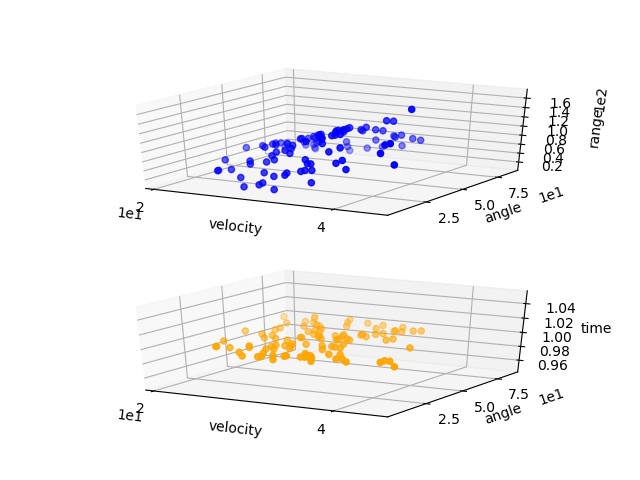
\includegraphics[scale=0.7]{../../tests/framework/user_guide/ForwardSamplingStrategies/gold/RunDir/SparseGrid/1-samplesModelPlot3D_scatter-scatter.png}
  \caption{Plot of validation samples generated by Monte Carlo sampling on the Code.}
  \label{fig:samplesSparseGridPlotModel}
 \end{figure}
 %%%%%%%%%%%%%%%%%%%%%%%%%%%%%%%%%%%%%%%%%%%%%%%%%%%%%%%%%%
   Finally, the previously defined \textbf{Entities} can be combined in
   the \xmlNode{Steps} block.
   The following \xmlNode{Steps} have been defined:
   \begin{itemize}
     \item \xmlNode{MultiRun} named ``sample'', used to run the training
     samples of the driven code and
     collect the outputs in the \textit{DataObjects}.
     The \xmlNode{Sampler} is specified to communicate to the
     \textit{Step} that the driven code needs to
     be sampled through the Sparse Grid Collocation sampling strategy;
     \item \xmlNode{RomTrainer} named ``train'', used to train (i.e.,
     construct) the GaussPolynomial ROM. This step is essential if the
     user want to use the ROM in later steps;
     \item \xmlNode{MultiRun} named ``sampleModel'', used to run the
     Monte Carlo perturbed samples of the original Model for use in verification.  The results are
     collected in the \textit{samplesModel} \textit{DataObjects}.
     \item \xmlNode{MultiRun} named ``sampleROM'', used to run the
     Monte Carlo perturbed samples of the previously constructed ROM for use in verificaiton.  The results are
     collected in the \textit{samplesROM} \textit{DataObjects}.
     \item \xmlNode{IOStep} named ``rom\_stas'', used to dump rom-related information into \textit{DataObject },
     \item  \xmlNode{IOStep} named ``output\_print'', used to dump
     the ``histories'', ``samplesModel'' and ``samplesROM'' \textit{DataObjects}
     \textbf{Entity} in a CSV file,
     \item  \xmlNode{IOStep} named ``output\_plot'', used to
     plot the data and store it in the PNG file and
     on the screen.
   \end{itemize}
\end{enumerate}
 % As previously mentioned, Figure~\ref{fig:historiesSparseGridPlotScatter}
 % shows the evolution of the outputs $A,B,C,D$ under uncertainties.
 % Figures~\ref{fig:samplesSparseGridPlotModel} and
 % \ref{fig:samplesROMSparseGridPlot} show the final responses
 % of the sampling employed using the driven code and the ROM,
 % respectively. 
 As it can be seen, the constructed ROM can accurately
 represent the response of the driven code. This example shows the
 potential of reduced order modeling, in general, and of the
 \textit{GaussPolynomialRom}, in particular.

  %%%%%%%%%%%%%%%%%%%%%%%%%%%%%%%%%%%%%%%%%%%%%%%%%%%%%%%%%%
 %figure samples
 \begin{figure}[h!]
  \centering
  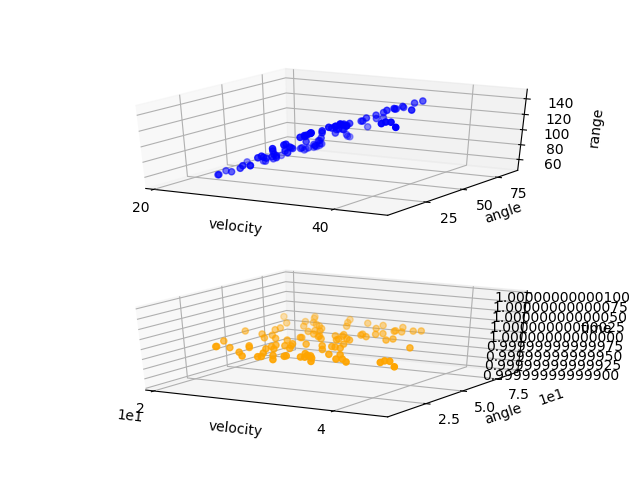
\includegraphics[scale=0.7]{../../tests/framework/user_guide/ForwardSamplingStrategies/gold/RunDir/SparseGrid/1-samplesROMPlot3D_scatter-scatter.png}
  \caption{Plot of validation samples generated by Monte Carlo sampling on the ROM.}
  \label{fig:samplesROMSparseGridPlot}
 \end{figure}
 %%%%%%%%%%%%%%%%%%%%%%%%%%%%%%%%%%%%%%%%%%%%%%%%%%%%%%%%%%









\section{Adaptive Sampling Strategies}
\label{sec:adaptiveSamplingStrategies}
Performing UQ and Dynamic PRA can be
challenging from a computational point of view. The \textit{Forward}
sampling strategies reported in the previous Section can lead to a large number of
unnecessary evaluations of the physical model leading to an unacceptable resource expenses (CPU time).
In addition, the \textit{Forward} methodologies are not designed to leverage the information
content that is extractable from the simulations already concluded.

To overcome these limitations, in RAVEN several adaptive algorithms are available:
\begin{enumerate}
  \item \textit{Limit Surface Search}
  \item \textit{Adaptive Dynamic Event Tree}
  \item \textit{Adaptive Hybrid Dynamic Event Tree}
  \item \textit{Adaptive Sparse Grid}
  \item \textit{Adaptive Sobol Decomposition}.
\end{enumerate}
In this Section, we will only show how to use the first algorithm.

%%%%%%%%%%%%%%%%
\subsection{Limit Surface Search sampling through RAVEN}
\label{sub:LSsamplingExample}
The goal of this Section is to learn how to:
 \begin{enumerate}
   \item Set up a LS Search sampling for efficiently perturb a driven code
   \item Use the LS Integral Post-processor for computing the probability of failure of the system subject to the same
   ``goal'' function
   \item Plot the obtained LS.
\end{enumerate}
In order to accomplish these tasks, the following RAVEN \textbf{Entities} (XML blocks in the input files) are defined:
\begin{enumerate}
   \item \textbf{\textit{RunInfo}}:
     \xmlExample[arg,extension,pauseAtEnd,overwrite]{framework/user_guide/AdaptiveSamplingStrategies/adaptiveSamplingLSsearch.xml}{RunInfo}
   As shown in Section~\ref{sub:EntitiesAndFlow}, the \textit{RunInfo} \textbf{Entity} is intended to set up the analysis
   that the user wants to perform. In this specific case, three steps (\xmlNode{Sequence}) are  sequentially run
   using eight processors (\xmlNode{batchSize}).
   \item \textbf{\textit{Files}}:
     \xmlExample[arg,extension,pauseAtEnd,overwrite]{framework/user_guide/AdaptiveSamplingStrategies/adaptiveSamplingLSsearch.xml}{Files}
   Since the driven code uses a single input file, in this Section the original input is placed. As detailed in the user manual
   the attribute  \xmlAttr{name} represents the alias that is going to be
   used in all the other input blocks in order to refer to this file.
   \\In addition the output file used in \xmlNode{Sequence}
   \textit{computeLSintegral} is here inputted.
   \item \textbf{\textit{Models}}:
     \xmlExample[arg,extension,pauseAtEnd,overwrite]{framework/user_guide/AdaptiveSamplingStrategies/adaptiveSamplingLSsearch.xml}{Models}
 As mentioned above, the goal of this example is the employment of
 an efficient sampling strategy, having as goal the determination of the
 failure of a system.

 In addition to the previously explained Code
 model,
 the ROM of type \textit{SciKitLearn} is here specified. The ROM will be
 used in the adaptive sampling strategy \textit{LimitSurfaceSearch} in
 order to accelerate the convergence of the method. As it can be seen,
 a nearest neighbor classifier is used, targeting only two uncertainties
 $sigma-A and decay-A$.
 \\ For the computation of the probability of failure (see the following), a
 Post-Processor (PP) of type \textit{LimitSurfaceIntegral} is here
 specified.This PP performs an integral of the LS
 generated by the adaptive sampling technique.
   \item \textbf{\textit{Distributions}}:
     \xmlExample{framework/user_guide/AdaptiveSamplingStrategies/adaptiveSamplingLSsearch.xml}{Distributions}
  In the Distributions XML Section, the stochastic model for the
  uncertainties  treated by the LS search sampling are reported. In
  this case two distributions are defined:
  \begin{itemize}
    \item $sigmaA \sim \mathbb{U}(0,1000)$, used to model the uncertainty
    associated with  the Model \textit{sigma-A}
    \item  $decayConstantA \sim \mathbb{U}(1e-8,1e-7)$,  used to
    model the uncertainty
    associated with  the Model \textit{decay-A}.
  \end{itemize}
   \item \textbf{\textit{Samplers}}:
     \xmlExample[arg,extension,pauseAtEnd,overwrite]{framework/user_guide/AdaptiveSamplingStrategies/adaptiveSamplingLSsearch.xml}{Samplers}
  In order to employ the LS search sampling strategy, a
  \xmlNode{LimitSurfaceSearch} node needs to be inputted.
  As it can be
  seen from above, each variable is associated to a different distribution
  defined in the  \xmlNode{Distributions} block.
  In addition, the \textit{AccelerationROM}  \xmlNode{ROM} is inputted.
  As already mentioned, this ROM (of type classifier) is used to
  accelerate the convergence of the LS Search method.
  In addition, the goal function \textit{goalFunction}  and the
  \textit{samples} are here reported.
  \\For this example, a convergence criterion of $1.0e-5$ is set. To reach such a confidence with a Monte-Carlo, millions of
  samples would be needed.
   \item \textbf{\textit{Functions}}:
     \xmlExample[arg,extension,pauseAtEnd,overwrite]{framework/user_guide/AdaptiveSamplingStrategies/adaptiveSamplingLSsearch.xml}{Functions}
 As already mentioned, the LS search sampling strategy uses
 a goal function in order to identify the regions of the uncertain space
 that are more informative. The \textit{goalFunction} used for this
 example is reported below. As it can be seen, if the final response $A$
 is $<=$ of $0.3$ , the system is considered to be in a ``safe'' condition.
\begin{lstlisting}[language=python]
def __residuumSign(self):
  returnValue = 1.0
  if self.A  <= 0.3:
    returnValue = -1.0
  return returnValue
\end{lstlisting}

   \item \textbf{\textit{DataObjects}}:
     \xmlExample[arg,extension,pauseAtEnd,overwrite]{framework/user_guide/AdaptiveSamplingStrategies/adaptiveSamplingLSsearch.xml}{DataObjects}
      In this block, three \textit{DataObjects} are defined: 1) PointSet
      named ``samples'' used to collect the final outcomes of the code, 2)
      HistorySet named ``histories'' in which the full time responses of the
      variables $A,B,C,D$ are going to be stored, 3) PointSet named
      ``limitSurface'' used  to export the LS location (in the uncertain space) during the employment of the sampling strategy.
   \item \textbf{\textit{OutStreams}}:
     \xmlExample[arg,extension,pauseAtEnd,overwrite]{framework/user_guide/AdaptiveSamplingStrategies/adaptiveSamplingLSsearch.xml}{OutStreams}
     Several out streams are included in this workflow, two for printing and three for plotting:
     \begin{itemize}
       \item ``samples'', which writes the validation sample contents of the \xmlString{samples} PointSet DataObject to a CSV file,
       \item ``histories'', which writes the sampling contents of the \xmlString{histories} HistorySet DataObject to a
         set of connected CSV files,
       \item ``historyPlot'', which plots the evolution of the samples taken,
       \item ``limitSurfacePlot'', which plots the limit surface discovered by the PostProcessor,
       \item ``samplesPlot3D'', which plots the final state of the samples taken against the figures of merit.
     \end{itemize}
     The plots demonstrate how visualization of three-dimensional data, time-dependent data, and limit
     surfaces can be realized using RAVEN.
 %%%%%%%%%%%%%%%%%%%%%%%%%%%%%%%%%%%%%%%%%%%%%%%%%%%%%%%%%%
 %%%%%%%%%%%%%%%%%%%%%%%%%%%%%%%%%%%%%%%%%%%%%%%%%%%%%%%%%%
 %figure samples
 \begin{figure}[h!]
  \centering
  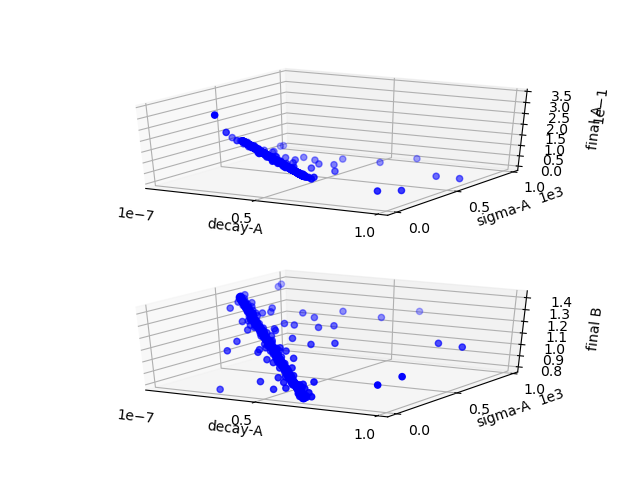
\includegraphics[scale=0.7]{../../tests/framework/user_guide/AdaptiveSamplingStrategies/gold/LSsearch/1-samplesPlot3D_scatter-scatter.png}
  \caption{Plot of the samples generated by the LS search sampling for variables $A,B$.}
  \label{fig:LS_pointsets}
 \end{figure}
 %%%%%%%%%%%%%%%%%%%%%%%%%%%%%%%%%%%%%%%%%%%%%%%%%%%%%%%%%%
 %%%%%%%%%%%%%%%%%%%%%%%%%%%%%%%%%%%%%%%%%%%%%%%%%%%%%%%%%%
   \item \textbf{\textit{Steps}}:
     \xmlExample[arg,extension,pauseAtEnd,overwrite]{framework/user_guide/AdaptiveSamplingStrategies/adaptiveSamplingLSsearch.xml}{Steps}
  %%%%%%%%%%%%%%%%%%%%%%%%%%%%%%%%%%%%%%%%%%%%%%%%%%%%%%%%%%
 %figure samples
 \begin{figure}[h!]
  \centering
  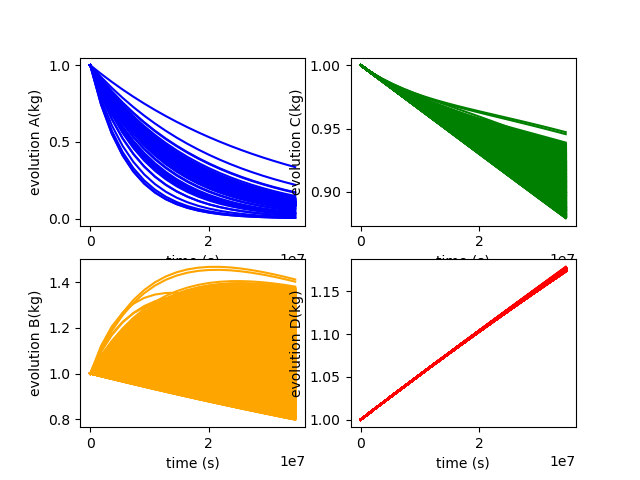
\includegraphics[scale=0.7]{../../tests/framework/user_guide/AdaptiveSamplingStrategies/gold/LSsearch/1-historyPlot_line-line-line-line.png}
  \caption{Plot of the histories generated by the LS search method for variables $A,B,C,D$.}
  \label{fig:LS_histories}
 \end{figure}
 %%%%%%%%%%%%%%%%%%%%%%%%%%%%%%%%%%%%%%%%%%%%%%%%%%%%%%%%%%
   Finally, all the previously defined \textbf{Entities} can be combined in
   the \xmlNode{Steps} block. As inferable,
   three \xmlNode{Steps} have been inputted:
   \begin{itemize}
     \item \xmlNode{MultiRun} named ``sample'', used to run the multiple
     instances of the driven code and
     collect the outputs in the two \textit{DataObjects}. As it can be
     seen, the \xmlNode{Sampler} is inputted to communicate to the
     \textit{Step} that the driven code needs to
     be perturbed through the LS search sampling strategy;
     \item \xmlNode{PostProcess} named ``computeLSintegral'', used to
     compute the probability of failure of the system based on the LS generated employing the LS search strategy. This
     probability is computed integrating the LS with a Monte-Carlo
     method.
     \item  \xmlNode{IOStep} named ``writeHistories'', used to 1) export
     the ``histories'' and ``samples''  \textit{DataObjects}
     \textbf{Entity} in a CSV file and 2) plot the data and the Limit Surface
     in  PNG files and on the screen.
   \end{itemize}
\end{enumerate}
 Figure~\ref{fig:LS_histories}
 shows the evolution of the outputs $A,B,C,D$ under uncertainties.
 Figure~\ref{fig:LS_pointsets} shows the final responses  of $A and B$
 of the sampling employed using the driven code.
 Figure~\ref{fig:LSplot}  shows the limit surface for this particular
 example. Only $367$ samples were needed in order to reach the full
 convergence.
 \\The integration of the LS determines a probability of failure of
 $~3.45e-2$.
  %%%%%%%%%%%%%%%%%%%%%%%%%%%%%%%%%%%%%%%%%%%%%%%%%%%%%%%%%%
 %figure samples
 \begin{figure}[h!]
  \centering
  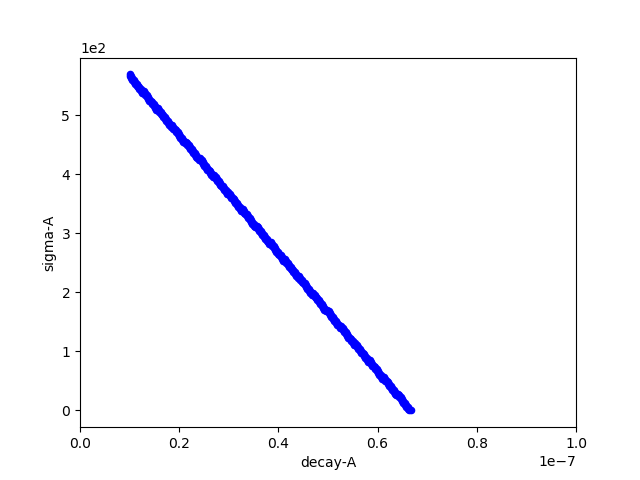
\includegraphics[scale=0.7]{../../tests/framework/user_guide/AdaptiveSamplingStrategies/gold/LSsearch/1-limitSurfacePlot_scatter.png}
  \caption{Limit Surface generated by the LS search method.}
  \label{fig:LSplot}
 \end{figure}
 %%%%%%%%%%%%%%%%%%%%%%%%%%%%%%%%%%%%%%%%%%%%%%%%%%%%%%%%%%









\input{restartSampling.tex}
\section{Reduced Order Modeling through RAVEN}
\label{sec:ROMraven}
The development of high-fidelity codes, for thermal-hydraulic systems
and integrated multi-physics, has undergone a significant acceleration
in the last years. Multi-physics codes simulate
multiple physical models or multiple simultaneous physical phenomena,
in a integrated solving environment. Multi-physics typically
solves coupled systems of partial differential equations, generally
characterized by several different geometrical and time scales.

The new multi-physics codes are characterized by remarkable
improvements
in the approximation of physics (high approximation order and reduced
use of empirical correlations). This greater fidelity is generally
accompanied by a greater computational effort (increased calculation time). This peculiarity is an
obstacle in the application of  computational techniques of
quantification of uncertainty and risk associated with the operation of
particular industrial plant (e.g., a nuclear reactor).

A solution to this problem is represented by the
usage
of highly effective sampling strategies. Sometimes also these
approaches is not enough
in order to perform a comprehensive UQ and PRA analysis. In these
cases the help of reduced order modeling is essential.

RAVEN has support of several different ROMs,
such as:
\begin{enumerate}
  \item \textit{Nearest Neighbors approaches}
  \item \textit{Support Vector Machines}
  \item \textit{Inverse Weight regressors}
  \item \textit{Spline regressors }, etc.
\end{enumerate}

A ROM, also known a surrogate
model, is a mathematical representation of a system, used to predict
a FOM of a physical system.

The ``training'' is a process of setting the internal parameters of the ROM from a set
of samples generated the physical model, i.e.,
 the high-fidelity simulator (RELAP-7, RELAP5
3D, PHISICS, etc.),
\begin{figure}[h!]
  \centering
  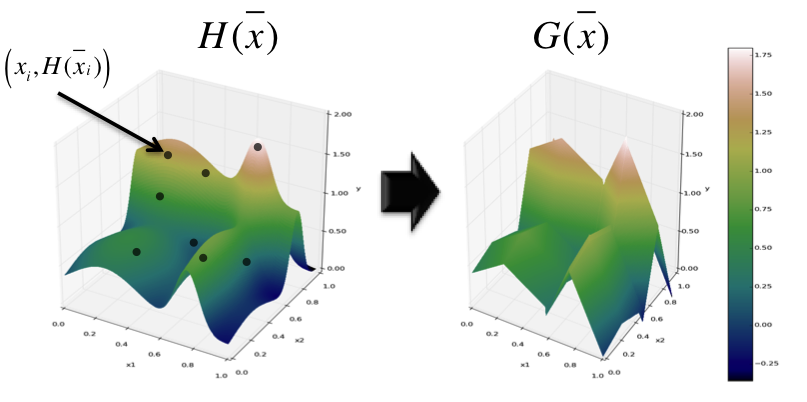
\includegraphics[width=1.0\textwidth]  {pics/ROMexampleOfPhysicalSystem.png}
  \caption{Example of reduced order model representation of physical system (regression).}
  \label{fig:ROMexampleOfPhysicalSystem}
\end{figure}

Two characteristics of these models
are generally assumed (even if exceptions are possible):
\begin{enumerate}
  \item The higher the number of realizations in the training sets, the
higher is the accuracy of the prediction performed by the ROM is. This
statement is true for most of the cases, although some ROMs might be
subject to the over-fitting issues. The over-fitting phenomenon is not
analyzed here, since its occurrence highly depends on the
algorithm type, and, hence, the problem needs to be analyzed for all
the large number of ROM types available
  \item The smaller the size of the input (uncertain) domain with
  respect to the variability of the system response, the more likely the
  ROM is able to represent the system response space.
\end{enumerate}

The goals of this section are about learning how to:
 \begin{enumerate}
   \item Set up a sampling strategy to construct multiple ROMs, perturbing a driven code
   \item Train the different ROMs with the data-set obtained by the applied sampling strategy;
   \item Use the same sampling strategy, perturbing the ROMs
   \item Plot the responses of the driven code and ROMs, respectively.
\end{enumerate}
In order to accomplish these tasks, the following RAVEN \textbf{Entities} (XML blocks in the input files) need to be defined:
\begin{enumerate}
   \item \textbf{\textit{RunInfo}}:
     \xmlExample{framework/user_guide/ReducedOrderModeling/reducedOrderModeling.xml}{RunInfo}
   As in the other examples, the the \textit{RunInfo} \textbf{Entity} is intended  to set up the analysis sequence that
   needs to be performed. The number of steps specified in (\xmlNode{Sequence}) are sequentially run, eight steps in this specific case, using the number of processors assigned in (\xmlNode{batchSize}).
   \\In the first step, the model is going to be sampled. The obtained results are going to be used to  train three different ROMs.These ROMs are sampled by the same strategy used in the first step in order to compare the ROMs' responses with the ones coming from the original model.
   \item \textbf{\textit{Models}}:
     \xmlExample{framework/user_guide/ReducedOrderModeling/reducedOrderModeling.xml}{Models}
 As mentioned earlier, the goal of this example is the employment of
 a sampling strategy in order to construct multiple types of ROMs.
 \\Indeed, in addition to an External model,
 three different ROMs (GP, SVM and IDW) are here specified. The ROMs will be
 constructed (``trained'') through the data-set generated by the sampling of the External model. Once trained, they are going  to be used in place of the original model.
 \\As it can be seen, the ROMs will be constructed considering two features ($v0,\, and angle,\,$) and two targets  ($r \, and \, t$).
   \item \textbf{\textit{Distributions}}:
     \xmlExample{framework/user_guide/ReducedOrderModeling/reducedOrderModeling.xml}{Distributions}
  In the Distributions XML section, the stochastic model for the
  uncertainties are reported. In
  this case two distributions are defined:
  \begin{itemize}
    \item $vel_dist \sim \mathbb{N}(30,5)$, used to model the uncertainties
    associated with  the \textit{velocity};
    \item  $angle_dist \sim \mathbb{U}(5,85)$,  used to
    model the uncertainties associated with the \textit{angle}.
  \end{itemize}
   \item \textbf{\textit{Samplers}}:
     \xmlExample{framework/user_guide/ReducedOrderModeling/reducedOrderModeling.xml}{Samplers}
  To obtain the data-set on which the data mining algorithms are going to be applied, a \textit{MonteCarlo} sampling approach is employed here.
   \item \textbf{\textit{DataObjects}}:
     \xmlExample{framework/user_guide/ReducedOrderModeling/reducedOrderModeling.xml}{DataObjects}
  Int this block, six \textit{DataObjects} are defined: 1) PointSet
  named ``samples'' used to collect the final outcomes of the code, 2)
  HistorySet named ``histories'' in which the full time responses of the
  variables are going to be stored, 3) PointSet named
  ``inputPlaceHolder'' used in the \textit{role} of \xmlNode{Input} for the ROMs sampling;
  4) PointSet named ``samplesGP'' used to collect the final outcomes (sampling) of the Gaussian Process (GP) ROM;
  5) PointSet named ``samplesInverse'' used to collect the final outcomes (sampling) of the Inverse Distance Weighting (IDW) ROM;
  6) PointSet named ``samplesSVM'' used to collect the final outcomes (sampling) of the Support Vector Machine (SVM) ROM.
 %%%%%%%%%%%%%%%%%%%%%%%%%%%%%%%%%%%%%%%%%%%%%%%%%%%%%%%%%%
 %%%%%%%%%%%%%%%%%%%%%%%%%%%%%%%%%%%%%%%%%%%%%%%%%%%%%%%%%%
 %figure samples
 \begin{figure}[h!]
  \centering
  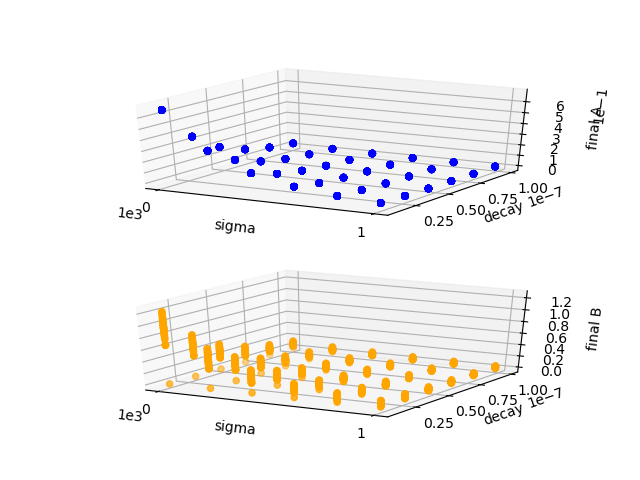
\includegraphics[scale=0.7]{../../tests/framework/user_guide/ReducedOrderModeling/gold/ROMConstruction/1-samplesPlot3D_scatter-scatter.png}
  \caption{Plot of the samples generated by the Monte Carlo sampling}
  \label{fig:ROMgrid_pointsets}
 \end{figure}
 %%%%%%%%%%%%%%%%%%%%%%%%%%%%%%%%%%%%%%%%%%%%%%%%%%%%%%%%%%
 %%%%%%%%%%%%%%%%%%%%%%%%%%%%%%%%%%%%%%%%%%%%%%%%%%%%%%%%%%
   \item \textbf{\textit{OutStreams}}:
     \xmlExample{framework/user_guide/ReducedOrderModeling/reducedOrderModeling.xml}{OutStreams}
     This model makes use of two Print OutStreams and five Plot OutStreams:
     \begin{itemize}
       \item ``samples,'' which writes the contents of the point-wise training samples to CSV,
       \item ``histories,'' which writes the contents of the history-wise training samples to linked CSVs,
       \item ``historyPlot,'' which plots the evolution of the training samples,
       \item ``samplesPlot3D,'' which plots the final state of the training samples with relation to the
         outputs of interest,
       \item ``samplesPlot3DROMgp,'' which plots the validation samples of the Gaussian Process ROM,
       \item ``samplesPlot3DROMsvm,'' which plots the validation samples of the Support-Vector Machine ROM,
       \item ``samplesPlot3Dinverse,'' which plots the validation samples of the multidimensional Inverse
         Weight ROM.
     \end{itemize}
     The 3D plots of the samples as well as the ROM samples can be used as a view-norm validation of the ROMs.
   \item \textbf{\textit{Steps}}:
     \xmlExample{framework/user_guide/ReducedOrderModeling/reducedOrderModeling.xml}{Steps}
  %%%%%%%%%%%%%%%%%%%%%%%%%%%%%%%%%%%%%%%%%%%%%%%%%%%%%%%%%%
 %figure samples
 \begin{figure}[h!]
  \centering
  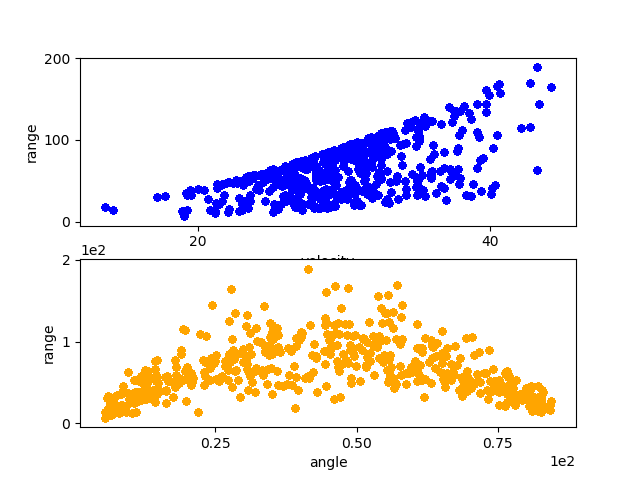
\includegraphics[scale=0.7]{../../tests/framework/user_guide/ReducedOrderModeling/gold/ROMConstruction/1-historyPlot_scatter-scatter.png}
  \caption{Plot of the histories generated by the Monte Carlo method}
  \label{fig:ROMgrid_histories}
 \end{figure}
   %%%%%%%%%%%%%%%%%%%%%%%%%%%%%%%%%%%%%%%%%%%%%%%%%%%%%%%%%%
 %figure samples
 \begin{figure}[h!]
  \centering
  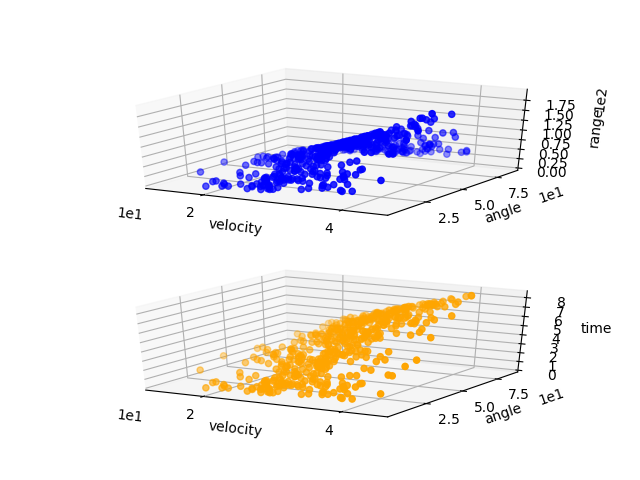
\includegraphics[scale=0.7]{../../tests/framework/user_guide/ReducedOrderModeling/gold/ROMConstruction/1-samplesPlot3DROMgp_scatter-scatter.png}
  \caption{Plot of the samples generated by the Monte Carlo sampling applied on the Gaussian Process ROM}
  \label{fig:ROMgp_samples}
 \end{figure}
 %%%%%%%%%%%%%%%%%%%%%%%%%%%%%%%%%%%%%%%%%%%%%%%%%%%%%%%%%%
 %%%%%%%%%%%%%%%%%%%%%%%%%%%%%%%%%%%%%%%%%%%%%%%%%%%%%%%%%%
   Finally, all the previously defined \textbf{Entities} can be combined in
   the \xmlNode{Steps} block. As inferable,
   eight \xmlNode{Steps} have been inputted:
   \begin{itemize}
     \item \xmlNode{MultiRun} named ``sample'', used to run the multiple
     instances of the driven code and
     collect the outputs in the two \textit{DataObjects}. As it can be
     seen, the \xmlNode{Sampler} is inputted to communicate to the
     \textit{Step} that the driven code needs to
     be perturbed through the Grid sampling strategy;
     \item \xmlNode{RomTrainer} named ``trainROMGaussianProcess'', used to construct (``train'')
     the GP ROM, based on the data-set generated in the  ``sample'' \textbf{Step};
     \item \xmlNode{RomTrainer} named ``trainROMsvm'', used to construct (``train'')
     the SVM ROM, based on the data-set generated in the  ``sample'' \textbf{Step};
     \item \xmlNode{RomTrainer} named ``trainROMinverse'', used to construct (``train'')
     the IDW ROM, based on the data-set generated in the  ``sample'' \textbf{Step};
     \item \xmlNode{MultiRun} named ``sampleROMGaussianProcess'', used to run the multiple
     instances of the previously constructed GP ROM and
     collect the outputs in the PointSet \textit{DataObject}. As it can be
     seen, the same \xmlNode{Sampler} used for perturbing the original model is here used.
     \item \xmlNode{MultiRun} named ``sampleROMsvm'', used to run the multiple
     instances of the previously constructed Support Vector Machine ROM and
     collect the outputs in the PointSet \textit{DataObject}. As it can be
     seen, the same \xmlNode{Sampler} used for perturbing the original model is here used.
     \item \xmlNode{MultiRun} named ``sampleROMInverse'', used to run the multiple
     instances of the previously constructed Inverse Distance Weight ROM and
     collect the outputs in the PointSet \textit{DataObject}. As it can be
     seen, the same \xmlNode{Sampler} used for perturbing the original model is here used.
     \item  \xmlNode{IOStep} named ``writeHistories'', used to 1) export
     the ``histories'' and ``samples''  \textit{DataObjects}
     \textbf{Entity} in a CSV file and 2) plot the responses of the sampling performed on the physical model, GP ROM,
     SVM ROM and IDW ROM in  PNG files and on the screen.
   \end{itemize}
\end{enumerate}

  %figure samples
 \begin{figure}[h!]
  \centering
  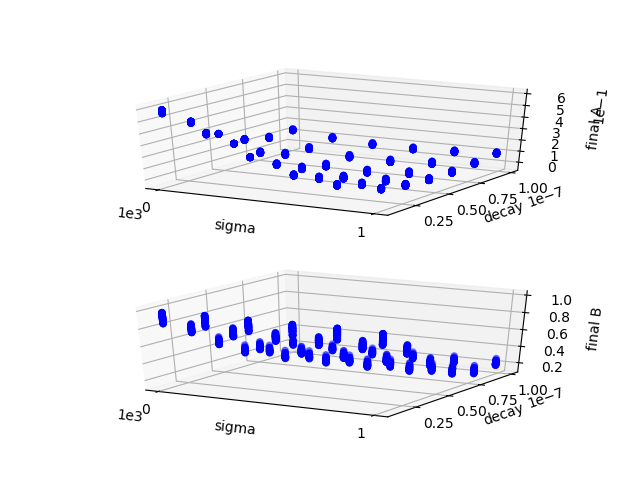
\includegraphics[scale=0.7]{../../tests/framework/user_guide/ReducedOrderModeling/gold/ROMConstruction/1-samplesPlot3DROMsvm_scatter-scatter.png}
  \caption{Plot of the samples generated by the Monte Carlo sampling applied on the Support Vector Machine ROM}
  \label{fig:ROMsvm_samples}
 \end{figure}
 %%%%%%%%%%%%%%%%%%%%%%%%%%%%%%%%%%%%%%%%%%%%%%%%%%%%%%%%%%
  %%%%%%%%%%%%%%%%%%%%%%%%%%%%%%%%%%%%%%%%%%%%%%%%%%%%%%%%%%
  %figure samples
 \begin{figure}[h!]
  \centering
  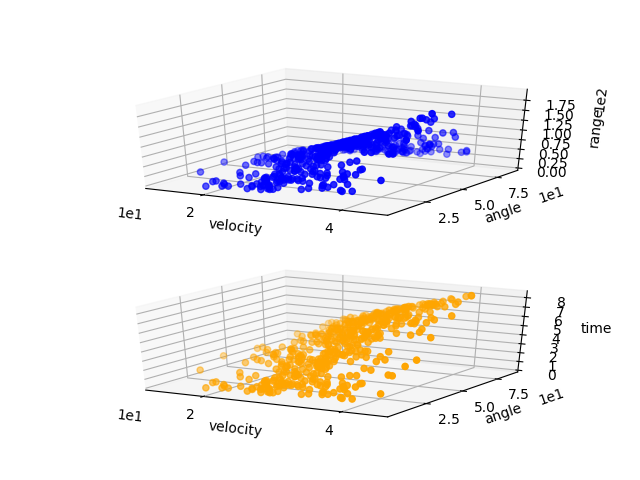
\includegraphics[scale=0.7]{../../tests/framework/user_guide/ReducedOrderModeling/gold/ROMConstruction/1-samplesPlot3DROMinverse_scatter-scatter.png}
  \caption{Plot of the samples generated by the Monte Carlo sampling applied on the Inverse Distance Weight ROM}
  \label{fig:ROMinverse_samples}
 \end{figure}
 %%%%%%%%%%%%%%%%%%%%%%%%%%%%%%%%%%%%%%%%%%%%%%%%%%%%%%%%%%
 Figure \ref{fig:ROMgrid_histories}
 shows the range $r$ for different velocity and angle.
 Figure \ref{fig:ROMgrid_pointsets} shows the final responses  of the sampling employed using the driven code.

Figures \ref{fig:ROMgp_samples}, \ref{fig:ROMsvm_samples} and \ref{fig:ROMinverse_samples}  show the final responses  of the sampling employed using the Gaussian Process, Support Vector Machines and Inverse Distance Weight ROMs, respectively.
It can be clearly noticed that the responses of the ROMs perfectly match the outcomes coming from the original model (see Figure   \ref{fig:ROMgrid_pointsets}).









\section{Statistical Analysis through RAVEN}
\label{sec:SAraven}
In order to perform a complete analysis of a system under uncertainties,
it is crucial to be able to compute all the statistical moments of one or even multiple
FOMs. In addition, it is essential to identify the correlation
among different FOMs toward a specific input space.

RAVEN is able to compute the most important statistical moments:
such as:
\begin{enumerate}
  \item \textit{Expected Value}
  \item \textit{Standard Deviation}
  \item \textit{Variance}
  \item \textit{variationCoefficient}
  \item \textit{Skewness}
  \item \textit{Kurtosis}
  \item \textit{Median}
  \item \textit{Percentile}.
\end{enumerate}
In addition, RAVEN fully supports the computation of all of the statistical moments defined to
``measure'' the correlation among variables/parameters/FOMs:
\begin{enumerate}
  \item \textit{Covariance matrix}
  \item \textit{Normalized Sensitivity matrix}
  \item \textit{Variance Dependent Sensitivity matrix}
  \item \textit{Sensitivity matrix}
  \item \textit{Pearson matrix}.
\end{enumerate}
The goals of this section is to show how to:
 \begin{enumerate}
   \item Set up a sampling strategy to perform a final statistical analysis
   perturbing a driven code
   \item Compute all the statistical moments and correlation/covariance
   metrics.
\end{enumerate}
In order to accomplish these tasks, the following RAVEN \textbf{Entities} (XML blocks in the input files) need to be defined:
\begin{enumerate}
   \item \textbf{\textit{RunInfo}}:
     \xmlExample{framework/user_guide/StatisticalAnalysis/statisticalAnalysis.xml}{RunInfo}
   As shown in the other examples, the \textit{RunInfo} \textbf{Entity} is intended  to set up the desired analysis. The number of steps specified in (\xmlNode{Sequence}) are sequentially run, two steps in this specific case, using the number of processors assigned in (\xmlNode{batchSize}).
   \\In the first step, the original physical model is sampled. The obtained results are  analyzed with the Statistical Post-Processor.
   \item \textbf{\textit{Models}}:
     \xmlExample{framework/user_guide/StatisticalAnalysis/statisticalAnalysis.xml}{Models}
 The goal of this example is to show how the
 principal statistical FOMs can be computed through RAVEN.
 \\We use an External model and specify a Post-Processor model (BasicStatistics). The post-process step is performed on all the output FOMs used in this example ($r and t$).
   \item \textbf{\textit{Distributions}}:
     \xmlExample{framework/user_guide/StatisticalAnalysis/statisticalAnalysis.xml}{Distributions}
  In the Distributions XML section, the stochastic model for the
  uncertainties are reported. In this case 2 distributions are defined:
  \begin{itemize}
    \item $vel\_dist \sim \mathbb{N}(30,5)$, used to model the uncertainties
    associated with  the \textit{velocity};
    \item  $angle\_dist \sim \mathbb{U}(5,85)$,  used to
    model the uncertainties associated with the \textit{angle}.
  \end{itemize}
   \item \textbf{\textit{Samplers}}:
     \xmlExample{framework/user_guide/StatisticalAnalysis/statisticalAnalysis.xml}{Samplers}
  In order to obtain the data-set on which the data mining algorithms are going to be applied, a \textit{MonteCarlo} sampling approach is employed here.
   \item \textbf{\textit{DataObjects}}:
     \xmlExample{framework/user_guide/StatisticalAnalysis/statisticalAnalysis.xml}{DataObjects}
  In this block, three \textit{DataObjects} are defined:
  1) PointSet named ``samples'' used to collect the final outcomes of
  the code,
  2) PointSet named ``dummyIN'' used as a placeholder for the \textit{Multirun} step,
  3) HistorySet named ``histories'' in which the full time responses of the
  variables $x,y,t$ are going to be stored.

   \item \textbf{\textit{Steps}}:
     \xmlExample{framework/user_guide/StatisticalAnalysis/statisticalAnalysis.xml}{Steps}

 %%%%%%%%%%%%%%%%%%%%%%%%%%%%%%%%%%%%%%%%%%%%%%%%%%%%%%%%%%
 %%%%%%%%%%%%%%%%%%%%%%%%%%%%%%%%%%%%%%%%%%%%%%%%%%%%%%%%%%
   Finally, all the previously defined \textbf{Entities} can be combined in
   the \xmlNode{Steps} block. As inferable,
   2 \xmlNode{Steps} have been inputted:
   \begin{itemize}
     \item \xmlNode{MultiRun} named ``sampleMC'', used to run the
     multiple
     instances of the driven code and
     collect the outputs in the two \textit{DataObjects}. As it can be
     seen, the \xmlNode{Sampler} is inputted to communicate to the
     \textit{Step} that the driven code needs to
     be perturbed through the MonteCarlo sampling strategy.
     \item \xmlNode{PostProcess} named ``statisticalAnalysisMC'', used
     compute all the statistical moments and FOMs based on the
     data obtained through the sampling strategy. As it can be noticed,
     the \xmlNode{Output} of the ``sampleMC'' \textit{Step} is the
     \xmlNode{Input} of the ``statisticalAnalysisMC''  \textit{Step}.
   \end{itemize}
\end{enumerate}

Tables \ref{ScalarMoments}-\ref{SensitivityComputed} show all the results of the \textit{PostProcess}
step.


\begin{table}[h!]
\centering
\caption{Computed Moments and Cumulants}
\label{ScalarMoments}
\begin{tabular}{|c|c|c|}
\hline
{\ul \textit{\textbf{Computed Quantities}}} & \textbf{r} & \textbf{t} \\ \hline
\textit{expected value}                     & 65.88   & 3.94   \\ \hline
\textit{median}                             & 61.74   & 4.12   \\ \hline
\textit{variance}                           & 1022.01 & 3.53   \\ \hline
\textit{sigma}                              & 31.97   & 1.89  \\ \hline
\textit{variation coefficient}              & 0.48    & 0.48   \\ \hline
\textit{skewness}                           & 0.55    & -0.03  \\ \hline
\textit{kurtosis}                           & -0.01   & -0.96  \\ \hline
\textit{percentile 5\%}                     & 20.21   & 0.85   \\ \hline
\textit{percentile 95\%}                    & 122.83  & 6.90   \\ \hline
\end{tabular}
\end{table}
\begin{table}[h!]
\centering
\caption{Covariance matrix.}
\label{covarianceComputed}
\begin{tabular}{|c|c|c|}
\hline
{\ul \textit{\textbf{Covariance}}} & \textbf{r} & \textbf{t} \\ \hline
\textit{velocity}                     & 95.36   & 3.29   \\ \hline
\textit{angle}                        & 25.29   & 40.42   \\ \hline
\end{tabular}
\end{table}
\begin{table}[h!]
\centering
\caption{Correlation matrix}
\label{pearsonComputed}
\begin{tabular}{|c|c|c|}
\hline
{\ul \textit{\textbf{Correlation}}} & \textbf{r} & \textbf{t} \\ \hline
\textit{velocity}                     & 0.61   & 0.36   \\ \hline
\textit{angle}                        & 0.03   & 0.92   \\ \hline
\end{tabular}
\end{table}
\begin{table}[h!]
\centering
\caption{Variance Dependent Sensitivity matrix}
\label{VarDepSensitivityComputed}
\begin{tabular}{|c|c|c|}
\hline
{\ul \textit{\textbf{Variance Sensitivity}}} & \textbf{r} & \textbf{t} \\ \hline
\textit{velocity}                     & -1.69   & 0.08   \\ \hline
\textit{angle}                        & -3.31   & 0.07   \\ \hline
\end{tabular}
\end{table}
\begin{table}[h!]
\centering
\caption{Sensitivity matrix}
\label{SensitivityComputed}
\begin{tabular}{|c|c|c|}
\hline
{\ul \textit{\textbf{Sensitivity (I/O)}}} & \textbf{r} & \textbf{t} \\ \hline
\textit{velocity}                     & 3.95   & 0.12   \\ \hline
\textit{angle}                        & 0.01   & 0.07   \\ \hline
\end{tabular}
\end{table}


\section{Data Mining through RAVEN}
\label{sec:DMraven}

Data mining is the computational process of discovering patterns in large data sets (``big data'') involving methods at the intersection of artificial intelligence, machine learning, statistics, and database systems. The overall goal of the data mining process is to extract information from a data set and transform it into an understandable structure for further use.
\\RAVEN has support of several different data mining algorithms,
such as:
\begin{enumerate}
  \item \textit{Hierarchical methodologies}
  \item \textit{K-Means}
  \item \textit{Mean-Shift}, etc.
\end{enumerate}

The goals of this section are about learning how to:
 \begin{enumerate}
   \item Set up a sampling strategy to apply clustering algorithms, perturbing a driven code
  \item Analyze the data using clustering algorithms.
\end{enumerate}
To accomplish these tasks, the following RAVEN \textbf{Entities} (XML blocks in the input files) need to be defined:
\begin{enumerate}
   \item \textbf{\textit{RunInfo}}:
     \xmlExample{framework/user_guide/DataMining/dataMiningAnalysis.xml}{RunInfo}
   The \textit{RunInfo} \textbf{Entity} is intended  to set up the analysis sequence that
   needs to be performed. The number of steps specified in (\xmlNode{Sequence}) are sequentially run
   using the number of processors assigned in (\xmlNode{batchSize}).
   \\In the first step, the original physical model is going to be sampled.
   The obtained results are going to be analyzed with data mining
   algorithms.
   \item \textbf{\textit{Models}}:
     \xmlExample{framework/user_guide/DataMining/dataMiningAnalysis.xml}{Models}
 The goal of this example is to show how the
 data mining algorithms in RAVEN can be useful to analyze large data set.
 \\In addition to an External model, two Post-Processor models ($DataMining|cluster|KMeans$ and $DataMining|decomposition|PCA$) are specified. Note that the post-processing is performed on all the output FOMs used in this example ($r and t$).
   \item \textbf{\textit{Distributions}}:
     \xmlExample{framework/user_guide/DataMining/dataMiningAnalysis.xml}{Distributions}
  In the Distributions XML section, the stochastic model for the
  uncertainties are reported. In this case 2 distributions are defined:
  \begin{itemize}
    \item $vel_dist \sim \mathbb{N}(30,5)$, used to model the uncertainties
    associated with  the \textit{velocity};
    \item  $angle_dist \sim \mathbb{U}(5,85)$,  used to
    model the uncertainties associated with the \textit{angle}.
  \end{itemize}
   \item \textbf{\textit{Samplers}}:
     \xmlExample{framework/user_guide/DataMining/dataMiningAnalysis.xml}{Samplers}
  In order to obtain the data-set on which the data mining algorithms are going to be applied, a \textit{MonteCarlo} sampling approach is employed here.
   \item \textbf{\textit{DataObjects}}:
     \xmlExample{framework/user_guide/DataMining/dataMiningAnalysis.xml}{DataObjects}
  In this block, three \textit{DataObjects} are defined:
  1) PointSet named ``samples'' used to collect the final outcomes of
  the code,
  2) PointSet named ``dummyIN'' used as a placeholder for the \textit{Multirun} step,
  3) HistorySet named ``histories'' in which the full time responses of the
  variables $x,y,t$ are going to be stored.
 %figure samples
 \begin{figure}[h!]
  \centering
  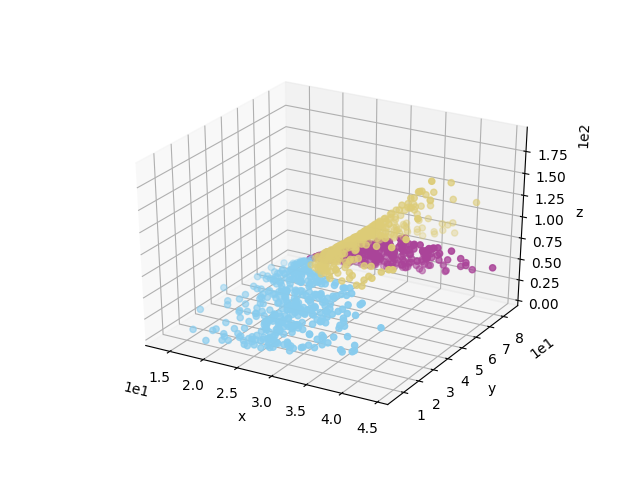
\includegraphics[scale=0.7]{../../tests/framework/user_guide/DataMining/gold/dataMiningAnalysis/1-PlotLabels_dataMining.png}
  \caption{K-means clustering on original dataset.}
  \label{fig:KmeanOrigData}
 \end{figure}
   \item \textbf{\textit{OutStreams}}:
     \xmlExample{framework/user_guide/DataMining/dataMiningAnalysis.xml}{OutStreams}
     This workflow uses one Print OutStream and three Plot OutStreams:
     \begin{itemize}
       \item ``samplesDump'', which writes the original sample set with the additional columns from the
         PostProcess steps,
       \item ``PlotKMeans1'', which plots the samples against the Figures of Merit with coloring according to the KMeans clustering,
       \item ``PlotLabels'', which plots the samples and colors them according to the KMeans clustering,
       \item ``PlotPCA1,'' which plots the surrogate principal component dimensions and their associated clustering.
     \end{itemize}
     Note that a special kind of plot, the ``dataMining'' \xmlNode{type}, has been implemented to simplify plotting complicated results using RAVEN, and is used in all three of the plots in this workflow.  Also note the use of the \xmlNode{range} block to define the data range of the plots created.
   \item \textbf{\textit{Steps}}:
     \xmlExample{framework/user_guide/DataMining/dataMiningAnalysis.xml}{Steps}

 %%%%%%%%%%%%%%%%%%%%%%%%%%%%%%%%%%%%%%%%%%%%%%%%%%%%%%%%%%
 %%%%%%%%%%%%%%%%%%%%%%%%%%%%%%%%%%%%%%%%%%%%%%%%%%%%%%%%%%
   Finally, all the previously defined \textbf{Entities} can be combined in
   the \xmlNode{Steps} block;
   3 \xmlNode{Steps} have been inputted:
   \begin{itemize}
     \item \xmlNode{MultiRun} named ``sample'', used to run the
     multiple
     instances of the driven code and
     collect the outputs in the two \textit{DataObjects}.The \xmlNode{Sampler} is inputted to communicate to the
     \textit{Step} that the driven code needs to
     be perturbed through the MonteCarlo sampling strategy;
     \item \xmlNode{PostProcess} named ``kmeans'', used
     to analyze the data obtained through the sampling strategy. In
     this step, a K-Means algorithm is going to be employed, plotting
     the clustering results;
     \textit{Step} that the driven code needs to
     be perturbed through the MonteCarlo sampling strategy;
     \item \xmlNode{PostProcess} named ``pca'', used
     to analyze the data obtained through the sampling strategy. In
     this Step, a PCA algorithm is going to be employed, plotting
     the decomposition results.
   \end{itemize}
\end{enumerate}
Figure~\ref{fig:KmeanOrigData} shows the clustering on the input space and the range, coloring according to the KMeans clustering,.
\\Figure~\ref{fig:KmeanProjected} shows the clustering on the range-angle and range-velocity plots respectively.
\\Figure~\ref{fig:PCAplot} shows the PCA decomposition on the data set.
%%%%%%%%%%%%%%%%%%%%%%%%%%%%%%%%%%%%%%%%%%%%%%%%%%%%%%%%%%
 %figure samples
 \begin{figure}[h!]
  \centering
  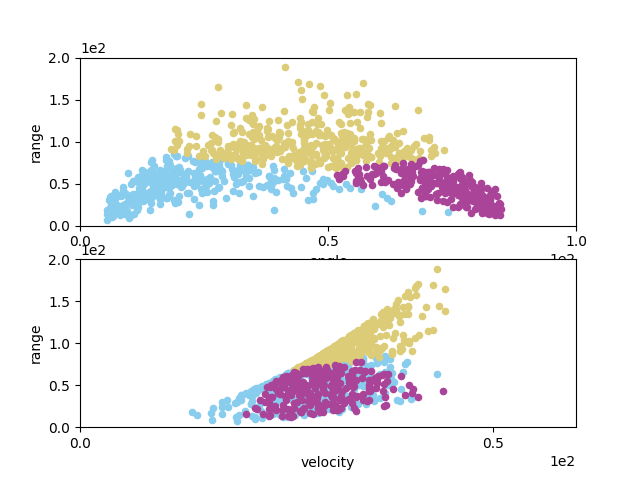
\includegraphics[scale=0.7]{../../tests/framework/user_guide/DataMining/gold/dataMiningAnalysis/1-PlotKMeans1_dataMining-dataMining.png}
  \caption{K-means clustering on projected parameters.}
  \label{fig:KmeanProjected}
 \end{figure}
 %%%%%%%%%%%%%%%%%%%%%%%%
 %%%%%%%%%%%%%%%%%%%%%%%%%%%%%%%%%%%%%%%%%%%%%%%%%%%%%%%%%%

 %%%%%%%%%%%%%%%%%%%%%%%%
  %%%%%%%%%%%%%%%%%%%%%%%%%%%%%%%%%%%%%%%%%%%%%%%%%%%%%%%%%%
 %figure samples
 \begin{figure}[h!]
  \centering
  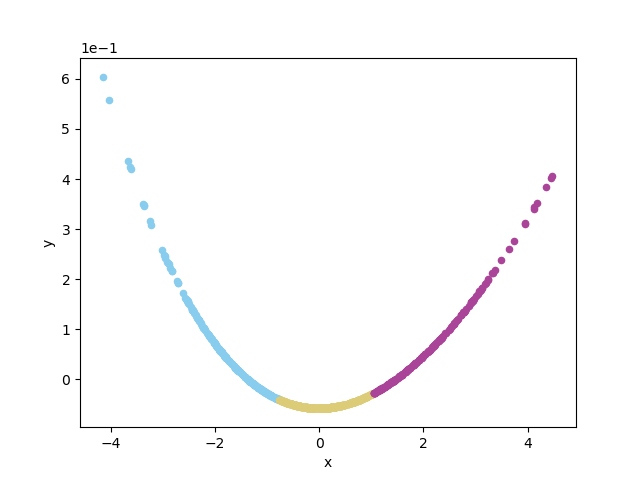
\includegraphics[scale=0.7]{../../tests/framework/user_guide/DataMining/gold/dataMiningAnalysis/1-PlotPCA1_dataMining.png}
  \caption{Principal Component Analysis.}
  \label{fig:PCAplot}
 \end{figure}
 %%%%%%%%%%%%%%%%%%%%%%%%


\clearpage
\begin{appendices}
  \section{Running RAVEN}
\label{HowToRun}

% I don't think this is mentioned earlier? Andrea answers :D It mentioned in the Introduction
%As already mentioned,
The RAVEN code is a blend of C++, C, and Python software. The entry point
resides on the Python side and is accessible via a command line interface.
%
After following the instructions in the previous Section, RAVEN is ready to be
used.
%
The \texttt{raven\_framework} script is in the raven folder.
%
To run RAVEN, open a terminal and use the following command (replace \texttt{<inputFileName.xml>} with your RAVEN input file):

\begin{itemize}

  \item \textbf{Any unix-based systems (e.g. Macintosh, Linux, etc.)}:
\begin{lstlisting}[language=bash]
raven_framework <inputFileName.xml>
\end{lstlisting}
  \item \textbf{Windows}:
  \begin{lstlisting}[language=bash]
bash.exe raven_framework <inputFileName.xml>
\end{lstlisting}
  
\end{itemize}

Using \texttt{raven\_framework} is the recommended way to run RAVEN.  In the event bypassing the typical
environment loading and checks is desired, it can also be run via
the \texttt{Driver.py} script using python, with the input file as argument.  However, this is not
recommended, as it will use whatever default versions of Python and other libraries are discovered, rather
than the matching libraries set up during installation.

\nb For Windows systems, we provided a convenient Batch script ( \texttt{raven\_framework.bat} ) for running RAVEN 
avoiding to interact with the Windows command line terminal. More info on how to use it can be found in the RAVEN
\wiki , section \textit{Running RAVEN} (\url{https://github.com/idaholab/raven/wiki/runningRAVEN}).


  \section{Document Version Information}
  \input{../version.tex}
\end{appendices}
%\appendix
\section{Appendix: Example Primer}
\label{sec:examplePrimer}
In this Appendix, a set of examples are reported. In order to be as general as possible, the \textit{Model} type ``ExternalModel'' has been used.
%%%% EXAMPLE 1
\subsection{Example 1.}
\label{subsec:ex1}
This simple example is about the construction of a ``Lorentz attractor'', sampling the relative input space. The parameters that are sampled represent the initial coordinate (x0,y0,z0) of the attractor origin.

\begin{lstlisting}[style=XML,morekeywords={debug,re,seeding,class,subType,limit}]
<?xml version="1.0" encoding="UTF-8"?>
<Simulation verbosity="debug">
<!-- RUNINFO -->
<RunInfo>
    <WorkingDir>externalModel</WorkingDir>
    <Sequence>FirstMRun</Sequence>
    <batchSize>3</batchSize>
</RunInfo>
<!-- Files -->
<Files>
    <Input name='lorentzAttractor.py' type=''>lorentzAttractor</Input>
</Files>
<!-- STEPS -->
<Steps>
    <MultiRun name='FirstMRun'  re-seeding='25061978'>
        <Input   class='Files'     type=''               >lorentzAttractor.py</Input>
        <Model   class='Models'    type='ExternalModel'  >PythonModule</Model>
        <Sampler class='Samplers'  type='MonteCarlo'     >MC_external</Sampler>
        <Output  class='DataObjects'     type='HistorySet'      >testPrintHistorySet</Output>
        <Output  class='Databases' type='HDF5'           >test_external_db</Output>
        <Output  class='OutStreams' type='Print'   >testPrintHistorySet_dump</Output>
    </MultiRun >
</Steps>
<!-- MODELS -->
<Models>
    <ExternalModel name='PythonModule' subType='' ModuleToLoad='externalModel/lorentzAttractor'>
       <variables>sigma,rho,beta,x,y,z,time,x0,y0,z0</variables>
    </ExternalModel>
</Models>
<!-- DISTRIBUTIONS -->
<Distributions>
    <Normal name='x0_distrib'>
        <mean>4</mean>
        <sigma>1</sigma>
    </Normal>
    <Normal name='y0_distrib'>
        <mean>4</mean>
        <sigma>1</sigma>
    </Normal>
    <Normal name='z0_distrib'>
        <mean>4</mean>
        <sigma>1</sigma>
    </Normal>
</Distributions>
<!-- SAMPLERS -->
<Samplers>
    <MonteCarlo name='MC_external'>
      <samplerInit>
        <limit>3</limit>
      </samplerInit>
      <variable name='x0' >
        <distribution  >x0_distrib</distribution>
      </variable>
      <variable name='y0' >
        <distribution  >y0_distrib</distribution>
      </variable>
      <variable name='z0' >
        <distribution  >z0_distrib</distribution>
      </variable>
    </MonteCarlo>
</Samplers>
<!-- DATABASES -->
<Databases>
  <HDF5 name="test_external_db"/>
</Databases>
<!-- OUTSTREAMS -->
<OutStreams>
  <Print name='testPrintHistorySet_dump'>
    <type>csv</type>
    <source>testPrintHistorySet</source>
  </Print>
</OutStreams>
<!-- DATA OBJECTS -->
<DataObjects>
    <HistorySet name='testPrintHistorySet'>
        <Input>x0,y0,z0</Input>
        <Output>time,x,y,z</Output>
   </HistorySet>
</DataObjects>
</Simulation>
\end{lstlisting}
The Python \textit{ExternalModel} is reported below:
\begin{lstlisting}[language=python]
import numpy as np

def run(self,Input):
  max_time = 0.03
  t_step = 0.01

  numberTimeSteps = int(max_time/t_step)

  self.x = np.zeros(numberTimeSteps)
  self.y = np.zeros(numberTimeSteps)
  self.z = np.zeros(numberTimeSteps)
  self.time = np.zeros(numberTimeSteps)

  self.x0 = Input['x0']
  self.y0 = Input['y0']
  self.z0 = Input['z0']

  self.x[0] = Input['x0']
  self.y[0] = Input['y0']
  self.z[0] = Input['z0']
  self.time[0]= 0

  for t in range (numberTimeSteps-1):
    self.time[t+1] = self.time[t] + t_step
    self.x[t+1]    = self.x[t] +  self.sigma*
                      (self.y[t]-self.x[t]) * t_step
    self.y[t+1]    = self.y[t] + (self.x[t]*
                      (self.rho-self.z[t])-self.y[t]) * t_step
    self.z[t+1]    = self.z[t] + (self.x[t]*
                          self.y[t]-self.beta*self.z[t]) * t_step
\end{lstlisting}
%%%% EXAMPLE 2
\subsection{Example 2.}
\label{subsec:ex1}
This example shows a slightly more complicated example, that employs the usage of:
\begin{itemize}
    \item \textit{Samplers:} Grid and Adaptive;
    \item \textit{Models:} External, Reduce Order Models and Post-Processors;
    \item \textit{OutStreams:} Prints and Plots;
    \item \textit{Data Objects:} PointSets;
    \item \textit{Functions:} ExternalFunctions.
\end{itemize}
The goal of this input is to compute the ``SafestPoint''.
It provides the coordinates of the farthest
point from the limit surface that is given as an input.
%
The safest point coordinates are expected values of the coordinates of the
farthest points from the limit surface in the space of the ``controllable''
variables based on the probability distributions of the ``non-controllable''
variables.

The term ``controllable'' identifies those variables that are under control
during the system operation, while the ``non-controllable'' variables are
stochastic parameters affecting the system behavior randomly.

The ``SafestPoint'' post-processor requires the set of points belonging to the
limit surface, which must be given as an input.

\begin{lstlisting}[style=XML,morekeywords={debug,re,seeding,class,subType,limit}]
<Simulation verbosity='debug'>

<!-- RUNINFO -->
<RunInfo>
  <WorkingDir>SafestPointPP</WorkingDir>
  <Sequence>pth1,pth2,pth3,pth4</Sequence>
  <batchSize>50</batchSize>
</RunInfo>

<!-- STEPS -->
<Steps>
  <MultiRun name = 'pth1' pauseAtEnd = 'False'>
    <Sampler  class = 'Samplers'  type = 'Grid'           >grd_vl_ql_smp_dpt</Sampler>
    <Input    class = 'DataObjects'     type = 'PointSet'   >grd_vl_ql_smp_dpt_dt</Input>
    <Model    class = 'Models'    type = 'ExternalModel'  >xtr_mdl</Model>
    <Output   class = 'DataObjects'     type = 'PointSet'   >nt_phy_dpt_dt</Output>
  </MultiRun >

  <MultiRun name = 'pth2' pauseAtEnd = 'True'>
    <Sampler          class = 'Samplers'  type = 'Adaptive'      >dpt_smp</Sampler>
    <Input            class = 'DataObjects'     type = 'PointSet'  >bln_smp_dt</Input>
    <Model            class = 'Models'    type = 'ExternalModel' >xtr_mdl</Model>
    <Output           class = 'DataObjects'     type = 'PointSet'  >nt_phy_dpt_dt</Output>
    <SolutionExport   class = 'DataObjects'     type = 'PointSet'  >lmt_srf_dt</SolutionExport>
  </MultiRun>

  <PostProcess name='pth3' pauseAtEnd = 'False'>
    <Input    class = 'DataObjects'          type = 'PointSet'       >lmt_srf_dt</Input>
    <Model    class = 'Models'         type = 'PostProcessor'  >SP</Model>
    <Output   class = 'DataObjects'          type = 'PointSet'     >sfs_pnt_dt</Output>
  </PostProcess>

  <OutStreamStep name = 'pth4' pauseAtEnd = 'True'>
  	<Input  class = 'DataObjects'            type = 'PointSet'  >lmt_srf_dt</Input>
  	<Output class = 'OutStreams' type = 'Print'         >lmt_srf_dmp</Output>
    <Input  class = 'DataObjects'            type = 'PointSet'  >sfs_pnt_dt</Input>
  	<Output class = 'OutStreams' type = 'Print'         >sfs_pnt_dmp</Output>
  </OutStreamStep>
</Steps>

<!-- DATA OBJECTS -->
<DataObjects>
  <PointSet name = 'grd_vl_ql_smp_dpt_dt'>
    <Input>x1,x2,gammay</Input>
    <Output>OutputPlaceHolder</Output>
  </PointSet>

  <PointSet name = 'nt_phy_dpt_dt'>
    <Input>x1,x2,gammay</Input>
    <Output>g</Output>
  </PointSet>

  <PointSet name = 'bln_smp_dt'>
    <Input>x1,x2,gammay</Input>
    <Output>OutputPlaceHolder</Output>
  </PointSet>

  <PointSet name = 'lmt_srf_dt'>
    <Input>x1,x2,gammay</Input>
    <Output>g_zr</Output>
  </PointSet>

  <PointSet name = 'sfs_pnt_dt'>
    <Input>x1,x2,gammay</Input>
    <Output>p</Output>
  </PointSet>
</DataObjects>

<!-- DISTRIBUTIONS -->
<Distributions>
  <Normal name = 'x1_dst'>
    <upperBound>10</upperBound>
    <lowerBound>-10</lowerBound>
  	<mean>0.5</mean>
    <sigma>0.1</sigma>
  </Normal>

  <Normal name = 'x2_dst'>
    <upperBound>10</upperBound>
    <lowerBound>-10</lowerBound>
    <mean>-0.15</mean>
    <sigma>0.05</sigma>
  </Normal>

  <Normal name = 'gammay_dst'>
    <upperBound>20</upperBound>
    <lowerBound>-20</lowerBound>
    <mean>0</mean>
    <sigma>15</sigma>
  </Normal>
</Distributions>

<!-- SAMPLERS -->
<Samplers>
  <Grid name = 'grd_vl_ql_smp_dpt'>
    <variable name = 'x1' >
      <distribution>x1_dst</distribution>
      <grid type = 'value' construction = 'equal' steps = '10' upperBound = '10'>2</grid>
    </variable>
    <variable name='x2' >
      <distribution>x2_dst</distribution>
      <grid type = 'value' construction = 'equal' steps = '10' upperBound = '10'>2</grid>
    </variable>
    <variable name='gammay' >
      <distribution>gammay_dst</distribution>
      <grid type = 'value' construction = 'equal' steps = '10' lowerBound = '-20'>4</grid>
    </variable>
  </Grid>

  <Adaptive name = 'dpt_smp' verbosity='debug'>
    <ROM              class = 'Models'    type = 'ROM'           >accelerated_ROM</ROM>
    <Function         class = 'Functions' type = 'External'      >g_zr</Function>
    <TargetEvaluation class = 'DataObjects'     type = 'PointSet'  >nt_phy_dpt_dt</TargetEvaluation>
    <Convergence limit = '3000' forceIteration = 'False' weight = 'none' persistence = '5'>1e-2</Convergence>
      <variable name = 'x1'>
        <distribution>x1_dst</distribution>
      </variable>
      <variable name = 'x2'>
        <distribution>x2_dst</distribution>
      </variable>
      <variable name = 'gammay'>
        <distribution>gammay_dst</distribution>
      </variable>
  </Adaptive>
</Samplers>

<!-- MODELS -->
<Models>
  <ExternalModel name = 'xtr_mdl' subType = '' ModuleToLoad = 'SafestPointPP/safest_point_test_xtr_mdl'>
    <variables>x1,x2,gammay,g</variables>
  </ExternalModel>

  <ROM name = 'accelerated_ROM' subType = 'SciKitLearn'>
    <Features>x1,x2,gammay</Features>
    <Target>g_zr</Target>
    <SKLtype>svm|SVC</SKLtype>
    <kernel>rbf</kernel>
    <gamma>10</gamma>
    <tol>1e-5</tol>
    <C>50</C>
  </ROM>

  <PostProcessor name='SP' subType='SafestPoint'>
    <!-- List of Objects (external with respect to this PP) needed by this post-processor -->
    <Distribution     class = 'Distributions'  type = 'Normal'>x1_dst</Distribution>
    <Distribution     class = 'Distributions'  type = 'Normal'>x2_dst</Distribution>
    <Distribution     class = 'Distributions'  type = 'Normal'>gammay_dst</Distribution>
    <!- end of the list -->
    <controllable>
    	<variable name = 'x1'>
    		<distribution>x1_dst</distribution>
    		<grid type = 'value' steps = '20'>1</grid>
    	</variable>
    	<variable name = 'x2'>
    		<distribution>x2_dst</distribution>
    		<grid type = 'value' steps = '20'>1</grid>
    	</variable>
    </controllable>
    <non-controllable>
    	<variable name = 'gammay'>
    		<distribution>gammay_dst</distribution>
    		<grid type = 'value' steps = '20'>2</grid>
    	</variable>
    </non-controllable>
  </PostProcessor>
</Models>

<!-- FUNCTIONS -->
<Functions>
  <External name='g_zr' file='SafestPointPP/safest_point_test_g_zr.py'>
    <variable>g</variable>
  </External>
</Functions>

<!-- OUT-STREAMS -->
<OutStreams>
  <Print name = 'lmt_srf_dmp'>
  	<type>csv</type>
  	<source>lmt_srf_dt</source>
  </Print>

  <Print name = 'sfs_pnt_dmp'>
  	<type>csv</type>
  	<source>sfs_pnt_dt</source>
  </Print>
</OutStreams>

</Simulation>
\end{lstlisting}
The Python \textit{ExternalModel} is reported below:
\begin{lstlisting}[language=python]
def run(self,Input):
  self.g = self.x1+4*self.x2-self.gammay
\end{lstlisting}
The ``Goal Function'',the function that defines the transitions with respect the input space coordinates, is as follows:
\begin{lstlisting}[language=python]
def __residuumSign(self):
  if self.g<0 : return  1
  else        : return -1
\end{lstlisting}

%%%%% EXAMPLE 3
%\subsection{Example3}
%\label{subsec:ex1}
%example 3



    % ---------------------------------------------------------------------- %
    % References
    %
    \clearpage
    % If hyperref is included, then \phantomsection is already defined.
    % If not, we need to define it.
    \providecommand*{\phantomsection}{}
    \phantomsection
    \addcontentsline{toc}{section}{References}
    \bibliographystyle{ieeetr}
    \bibliography{raven_user_guide}


    % ---------------------------------------------------------------------- %
    %

    % \printindex

    %\include{distribution}

\end{document}
